\vspace{-.5em}
\section{Results}
\label{exp}
We evaluate SVC first on a single node MySQL database to evaluate its accuracy, performance, and efficiency in a variety of materialized view 
scenarios.
We look at three main applications, join view maintenance, aggregate view maintenance, and a data cube application, on the standard TPCD benchmark 
and skewed version of the benchmark TPCD-Skew.
Then, we evaluate the outlier indexing approach in terms of improved query accuracy and also evaluate the overhead associated with using the index.
After evaluation on the benchmark, we present an end-to-end application of log analysis with a dataset from a video streaming company.
In this application, we look at the real query workload of the company and materialize views that could improve performance of these queries.
We implement SVC in Spark 1.1 and deploy it on a 10-node cluster to analyze 1TB of logs.

\subsection{Single-node Experimental Setup}
Our single node experiments are run on a r3.large Amazon EC2 node (2x Intel Xeon E5-2670, 15.25 GB Memory, and 32GB SSD Disk) with a MySQL version 5.6.15 database.
These experiments evaluate views from 10GB TPCD and TPCD-Skew datasets.
TPCD-Skew dataset \cite{tpcdskew} is based on the Transaction Processing Council's benchmark
schema but is modified so that it generates a dataset with values drawn from a Zipfian distribution instead of uniformly.
The Zipfian distribution \cite{mitzenmacher2004brief} is a long-tailed distribution with a single parameter $z=\{1,2,3,4\}$ which a larger
value means a more extreme tail.
$z=1$ corresponds to the basic TPCD benchmark. 
We implement incremental view maintenance with a \textbf{update...on duplicate key insert} command.
We implement SVC's sampling operator with a linear hash writter in C that is evoked in MySQL as a stored procedure.
In all of the applications, the updates are kept in memory in a temporary table, and we discount this loading time from our experiments.

Below we describe the view definitions and the queries on the views:

\textbf{Join View: } In the TPCD specification, two tables recieve insertions and updates: \textbf{lineitem} and \textbf{orders}.
Out of 22 parameterized queries in the specification, 12 are group-by aggregates of the join of \textbf{lineitem} and \textbf{orders} (Q3, Q4, Q5, Q7, Q8, Q9, Q10, Q12, Q14, Q18, Q19, Q21).
Therefore, we define a materialized view of the foreign-key join of \textbf{lineitem} and \textbf{orders}, and compare incremental view maintenance and SVC.
We treat the 12 group-by aggregates as queries on the view.

\textbf{Data Cube: } Another application which is common in industry analytics is data cubing.
We define the following ``base cube" as a materialized view that calculates the total revenue 
grouped by distinct customer, nation, region, and part number.
\begin{lstlisting}
select
  sum(l_extendedprice * (1 - l_discount)) as revenue,
  c_custkey, n_nationkey,
  r_regionkey, L_PARTKEY
from
  lineitem, orders,
  customer, nation,
  region
where
  l_orderkey = o_orderkey and
  O_CUSTKEY = c_custkey and
  c_nationkey = n_nationkey and
  N_REGIONKEY = r_regionkey

group by
  c_custkey, n_nationkey, 
  r_regionkey, L_PARTKEY
\end{lstlisting}
The queries on this view are ``rollup" queries that aggregate over 
subsets of the groups (eg. total of all customers in North America).

\textbf{Queries as View: } Finally, to test the generality of SVC, we treat each of the 22 queries in TPCD as a materialized view.
10 out of the 22 can benefit from SVC (see table ??).
As each of the queries are actually parameterized queries, we generated 10 views for each TPCD query.
For each of the views, we generated \emph{queries on the views}.
We generated 100 random aggregate queries for each view.
We detail the incremental maintenance procedures in ??.

\subsubsection{Distributed Experimental Setup}
We evaluated performance on Apache Spark 1.1.0 with a 10 node r3.large Amazon EC2 cluster.
Spark supports materialized views through a distributed data structure called an RDD \cite{zaharia2012resilient}.
There is a SQL interface which transforms the RDD's using Map-Reduce chains.
As RDD's are an immutable data structure, any maintenance must be done synchronously.
As Spark aslo does not have support for indices, we rely on partitioned joins for incremental maintenance of the views.
We partitioned the views by primary-by key, and apply a full outer join of the updates with the partitioned view.

We evalaute SVC on a 1TB dataset of logs from Conviva \cite{conviva}.
Conviva is a video streaming company and we evaluated our approach on user activity logs.
1TB corresponded to a sample of customer data from 1 year of logs.
With this dataset, there was a corresponding dataset of analyst SQL queries on the log table.
We used this dataset to evaluate the end-to-end accuracy and performance of the system in a real-world application.

Using the dataset of analyst queries, we identified 8 common summary statistics-type queries that calculated engagement and error-diagnosis metrics for specific customers on a certain day.
We generalized these queries by turning them into group-by queries over customers and dates; that is a view that calculates the metric for every customer on every day.
We generated aggregate random queries over this dataset by taking either random time ranges or random subsets of customers.

\subsection{Single-node Accuracy and Performance}

\subsubsection{Join View}
\begin{figure}[t]
\centering
 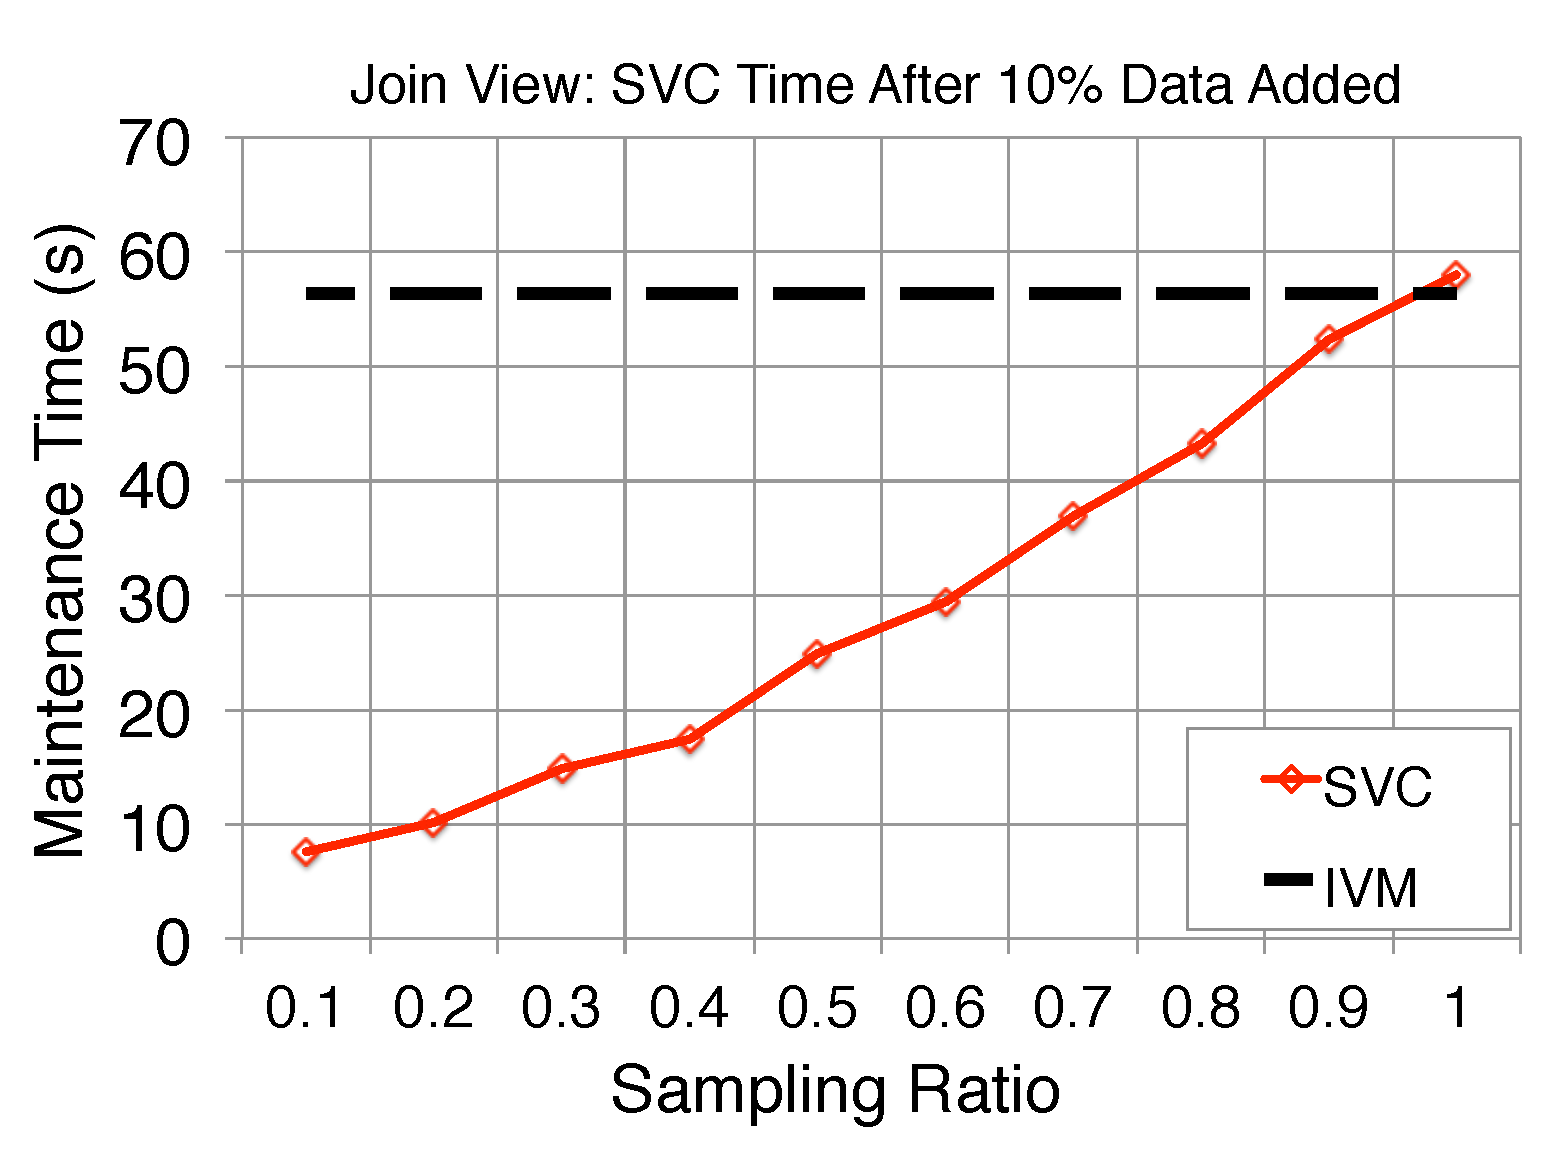
\includegraphics[scale=0.15]{exp/msj_1.pdf}
 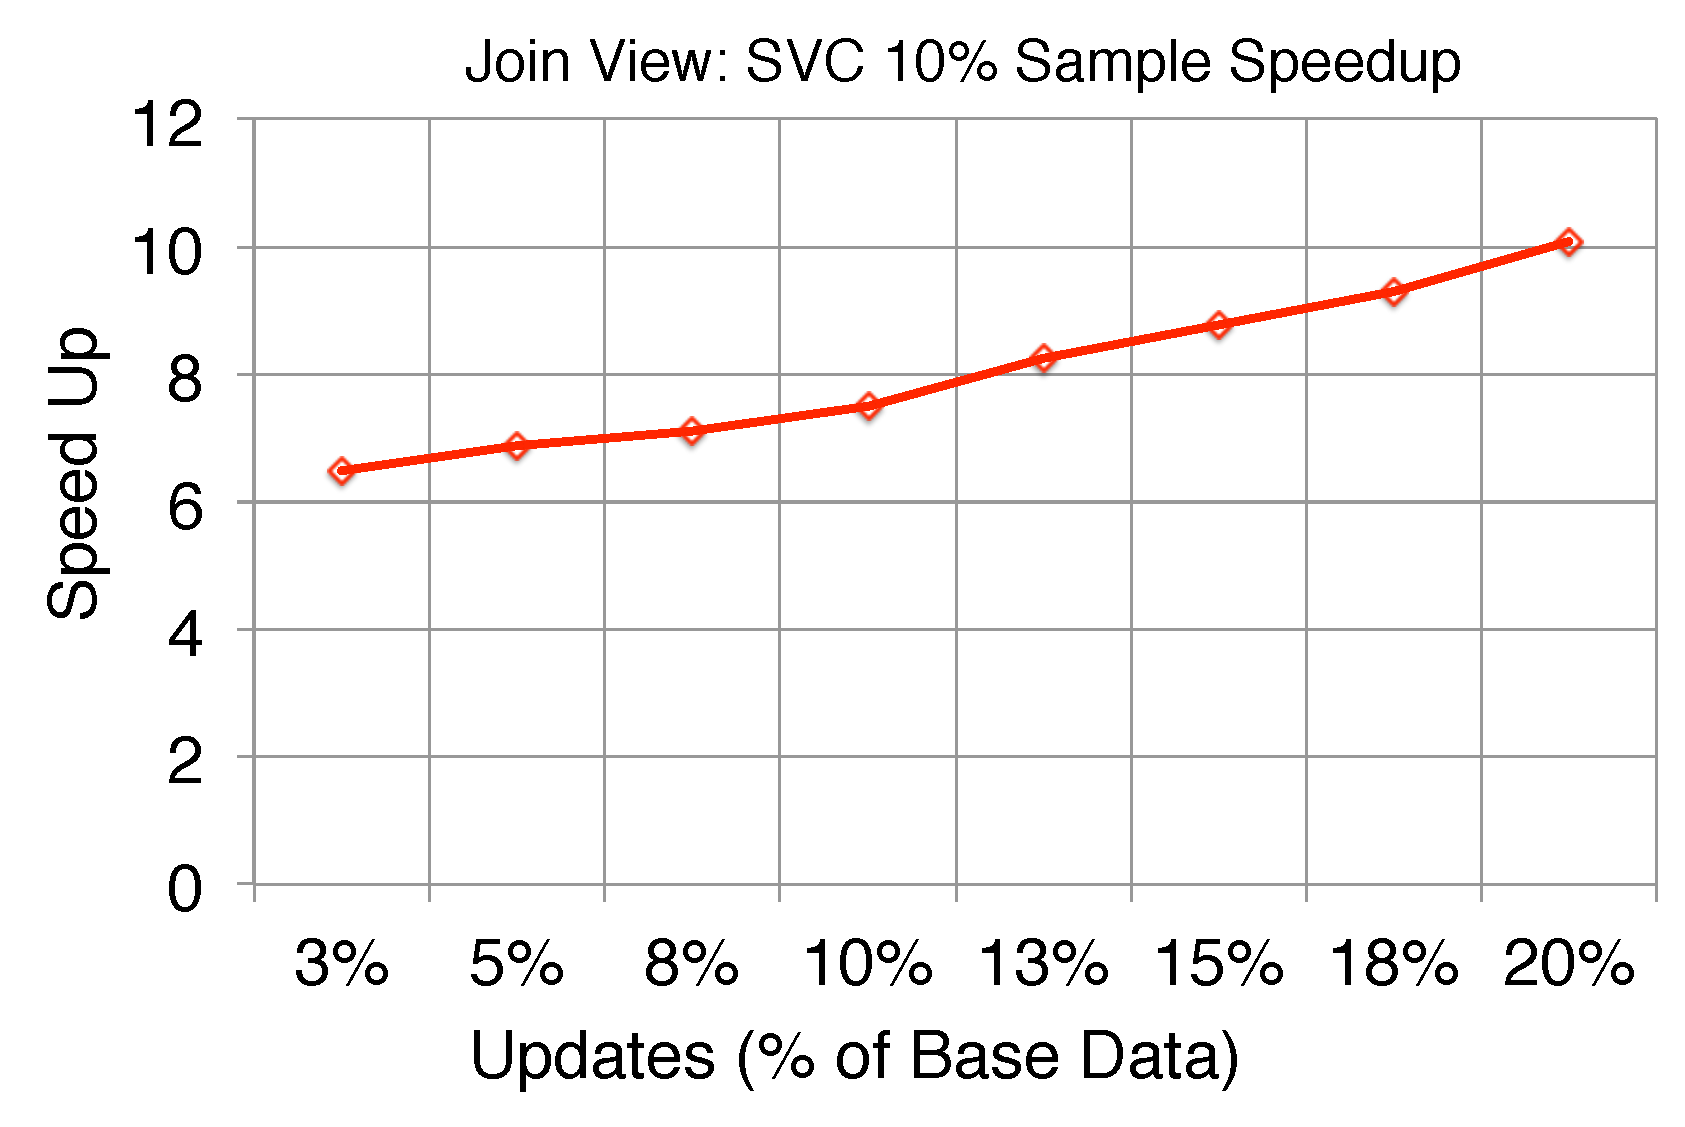
\includegraphics[scale=0.15]{exp/msj_2.pdf}
 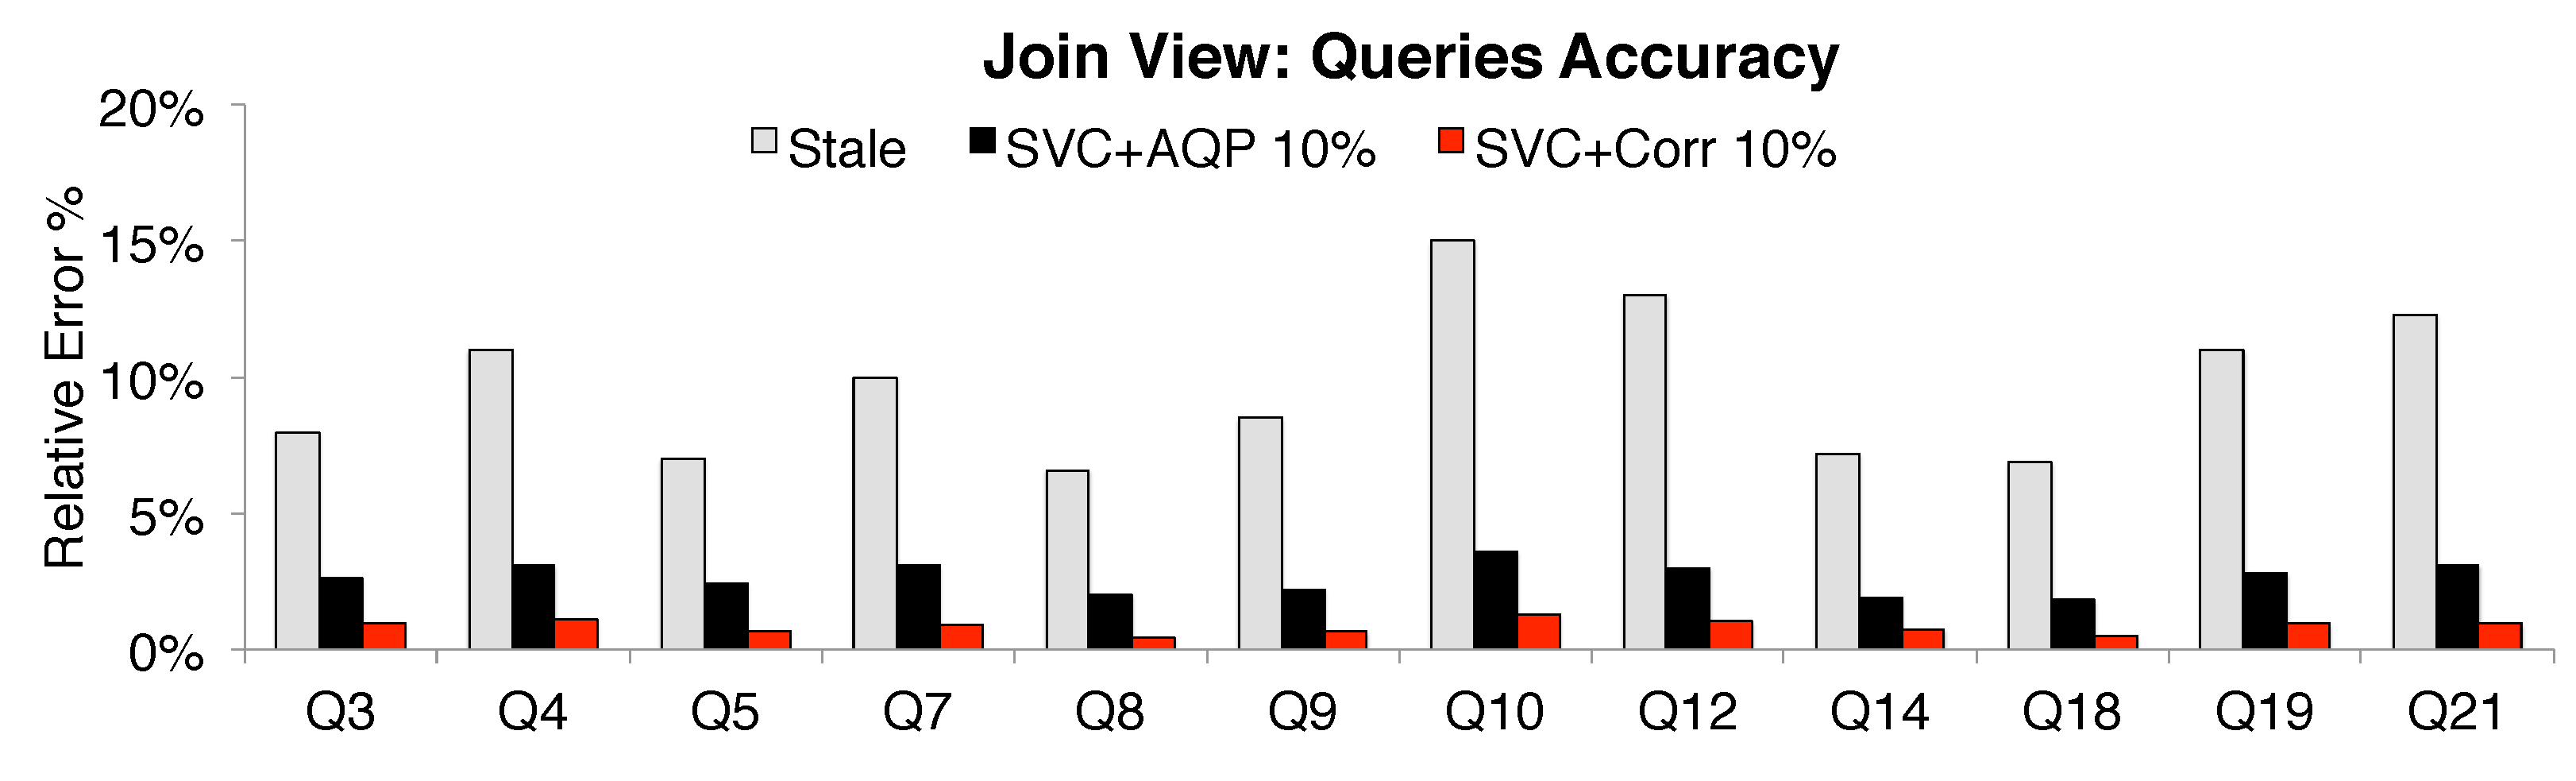
\includegraphics[scale=0.16]{exp/msj_3.pdf}
 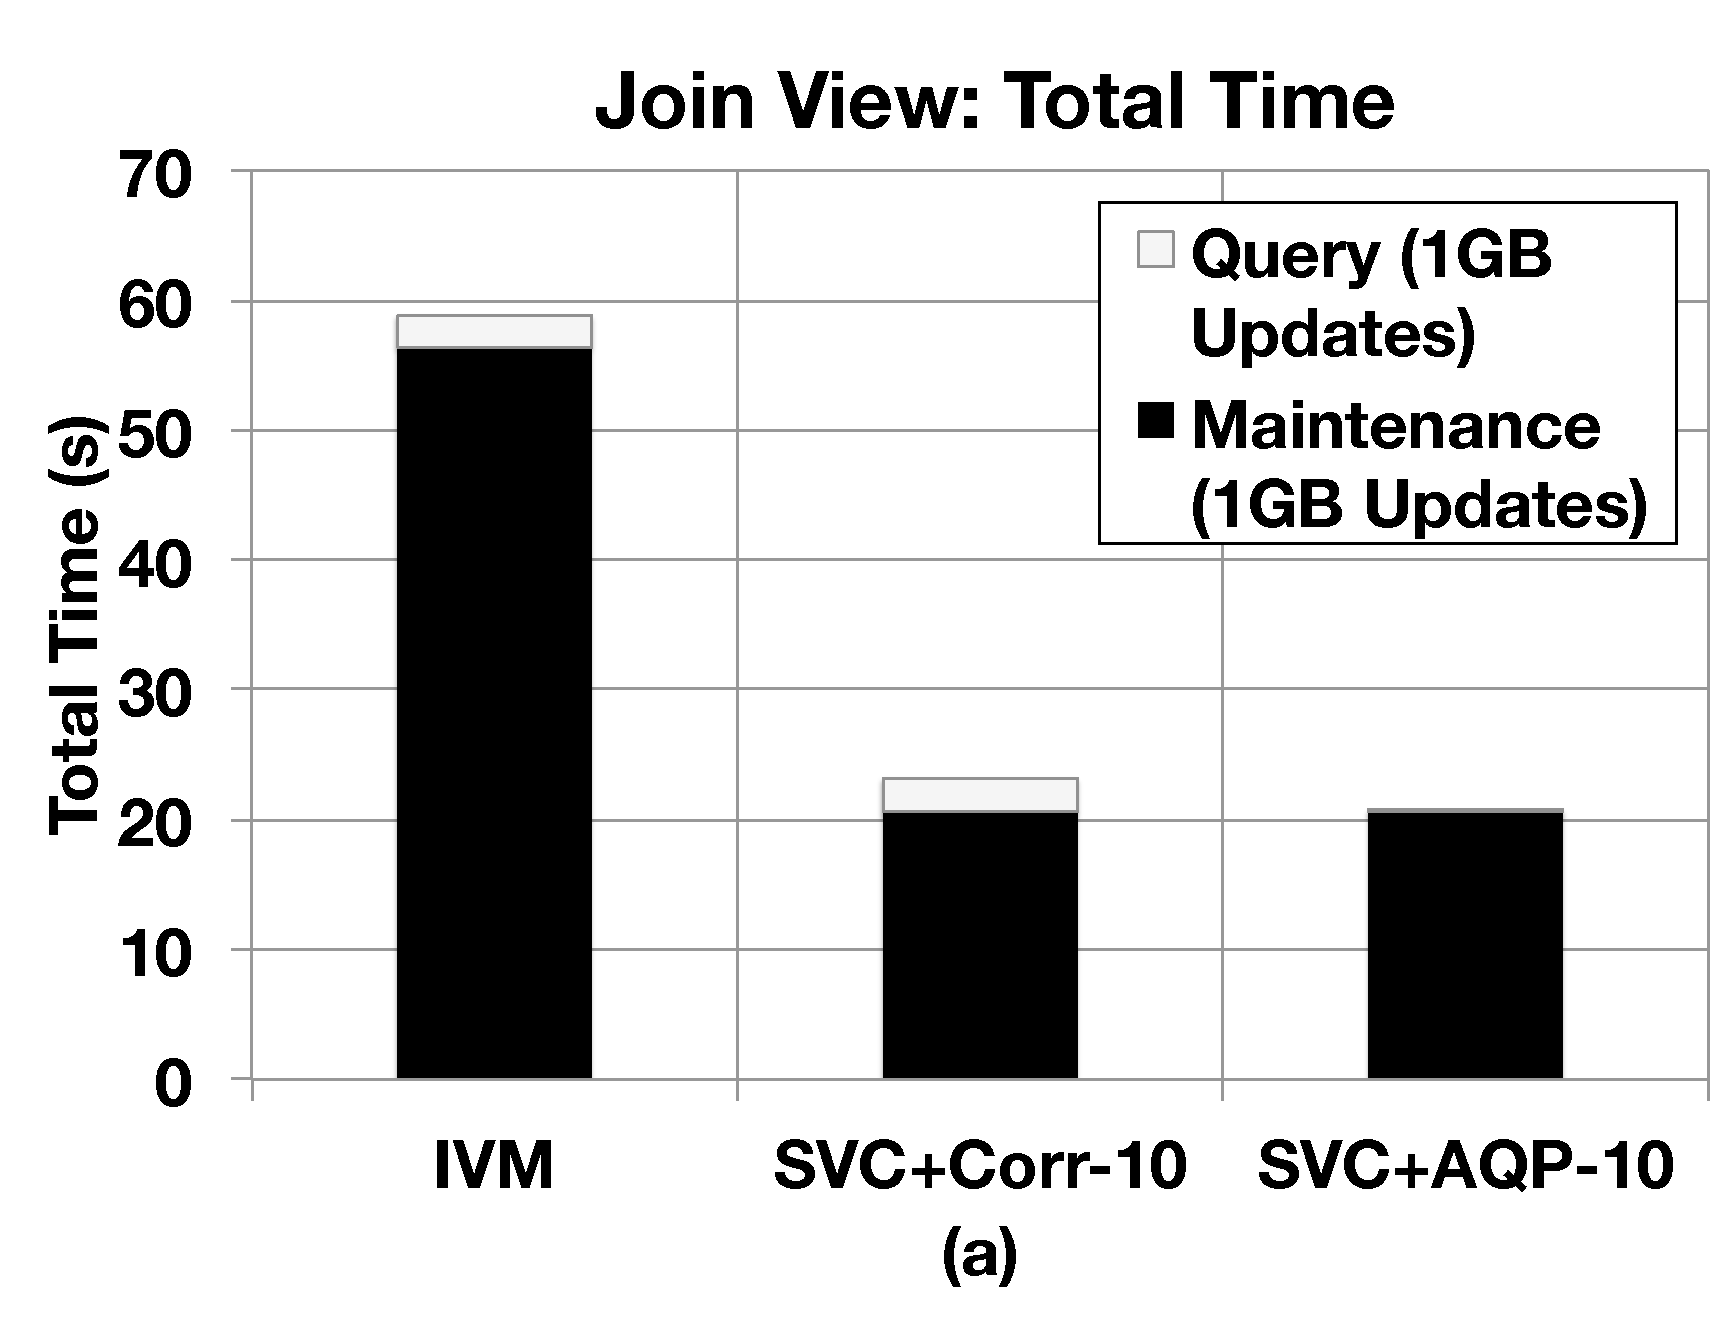
\includegraphics[scale=0.16]{exp/msj_4.pdf}
  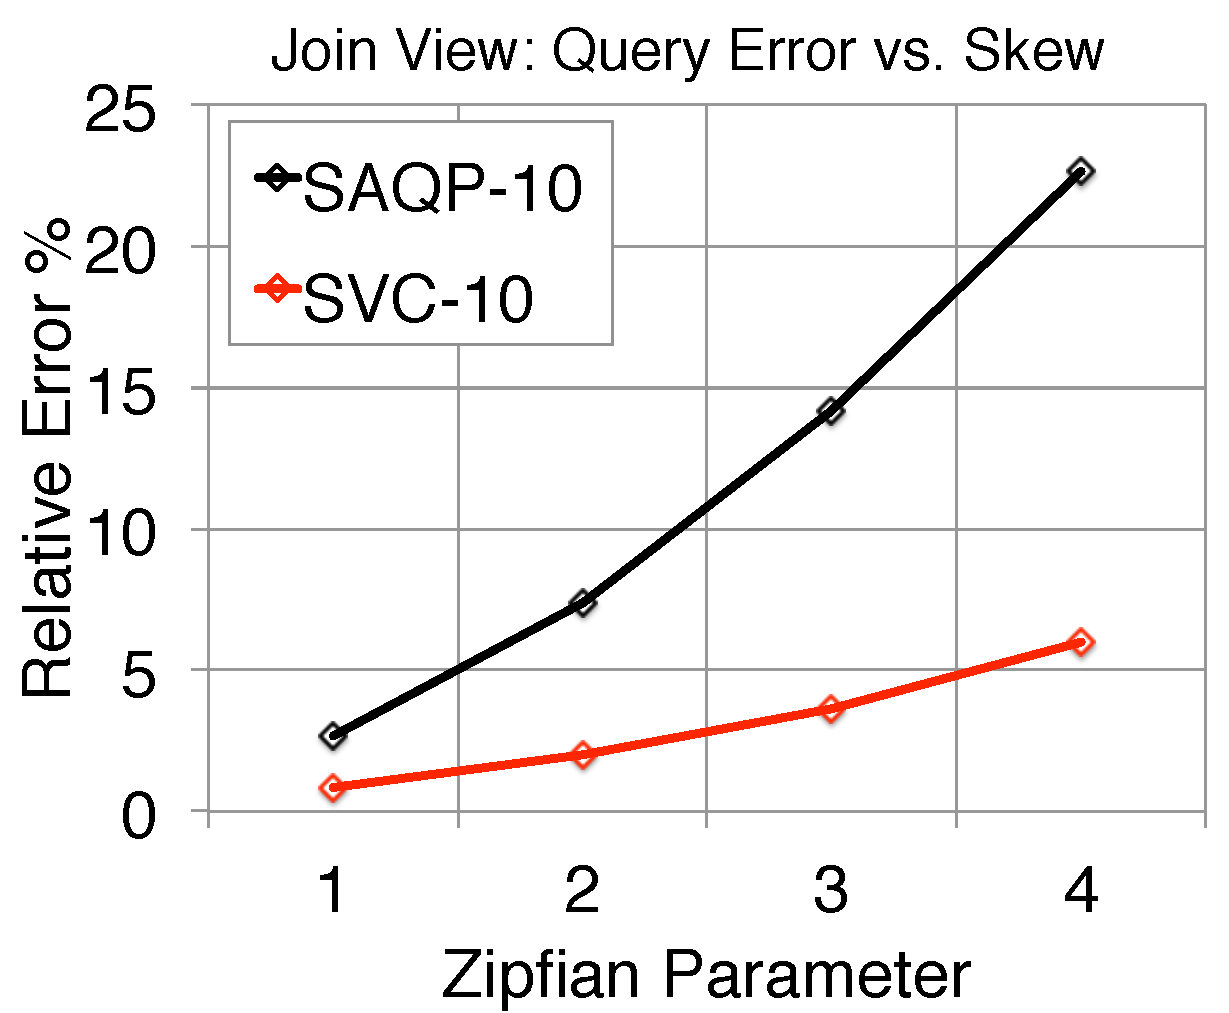
\includegraphics[scale=0.15]{exp/msj_5.pdf}
 \caption{TODO}
\end{figure}

\subsubsection{Data Cube View}
\begin{figure}[t]
\centering
 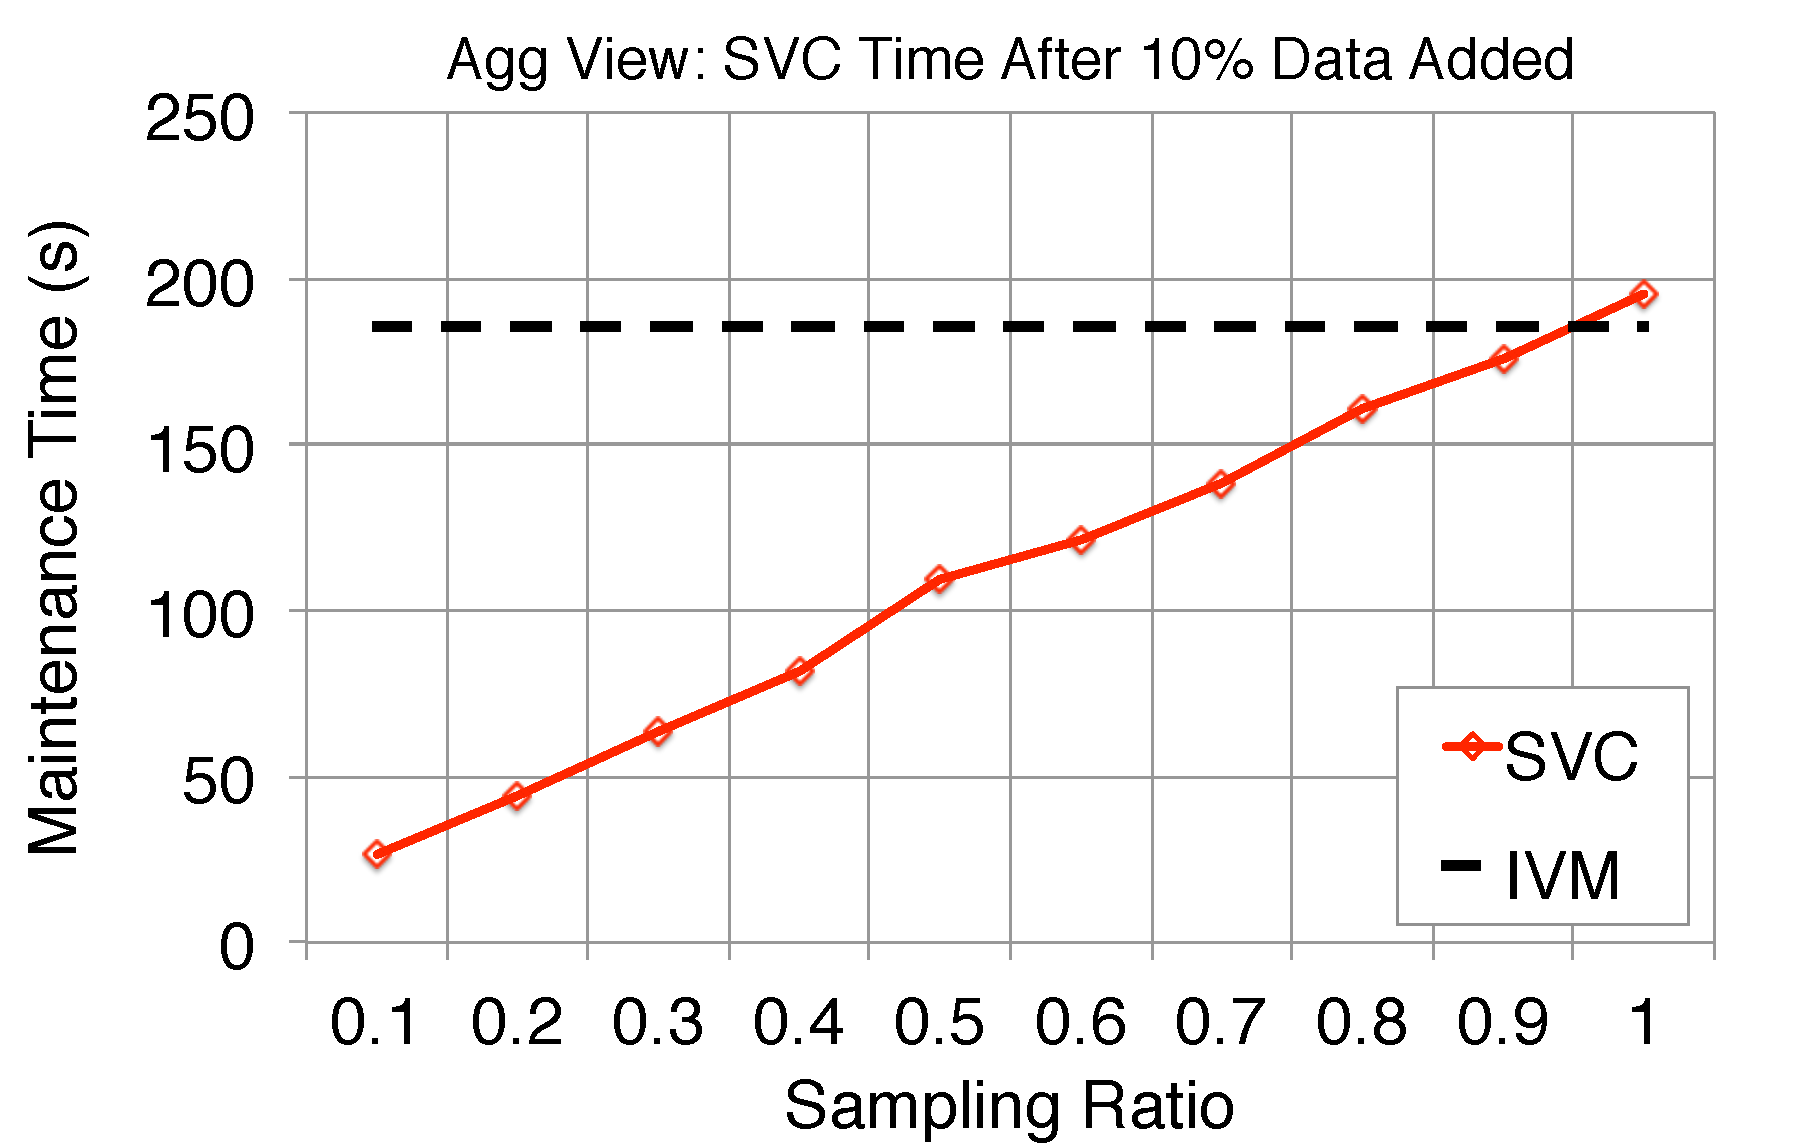
\includegraphics[scale=0.14]{exp/msdc_1.pdf}
 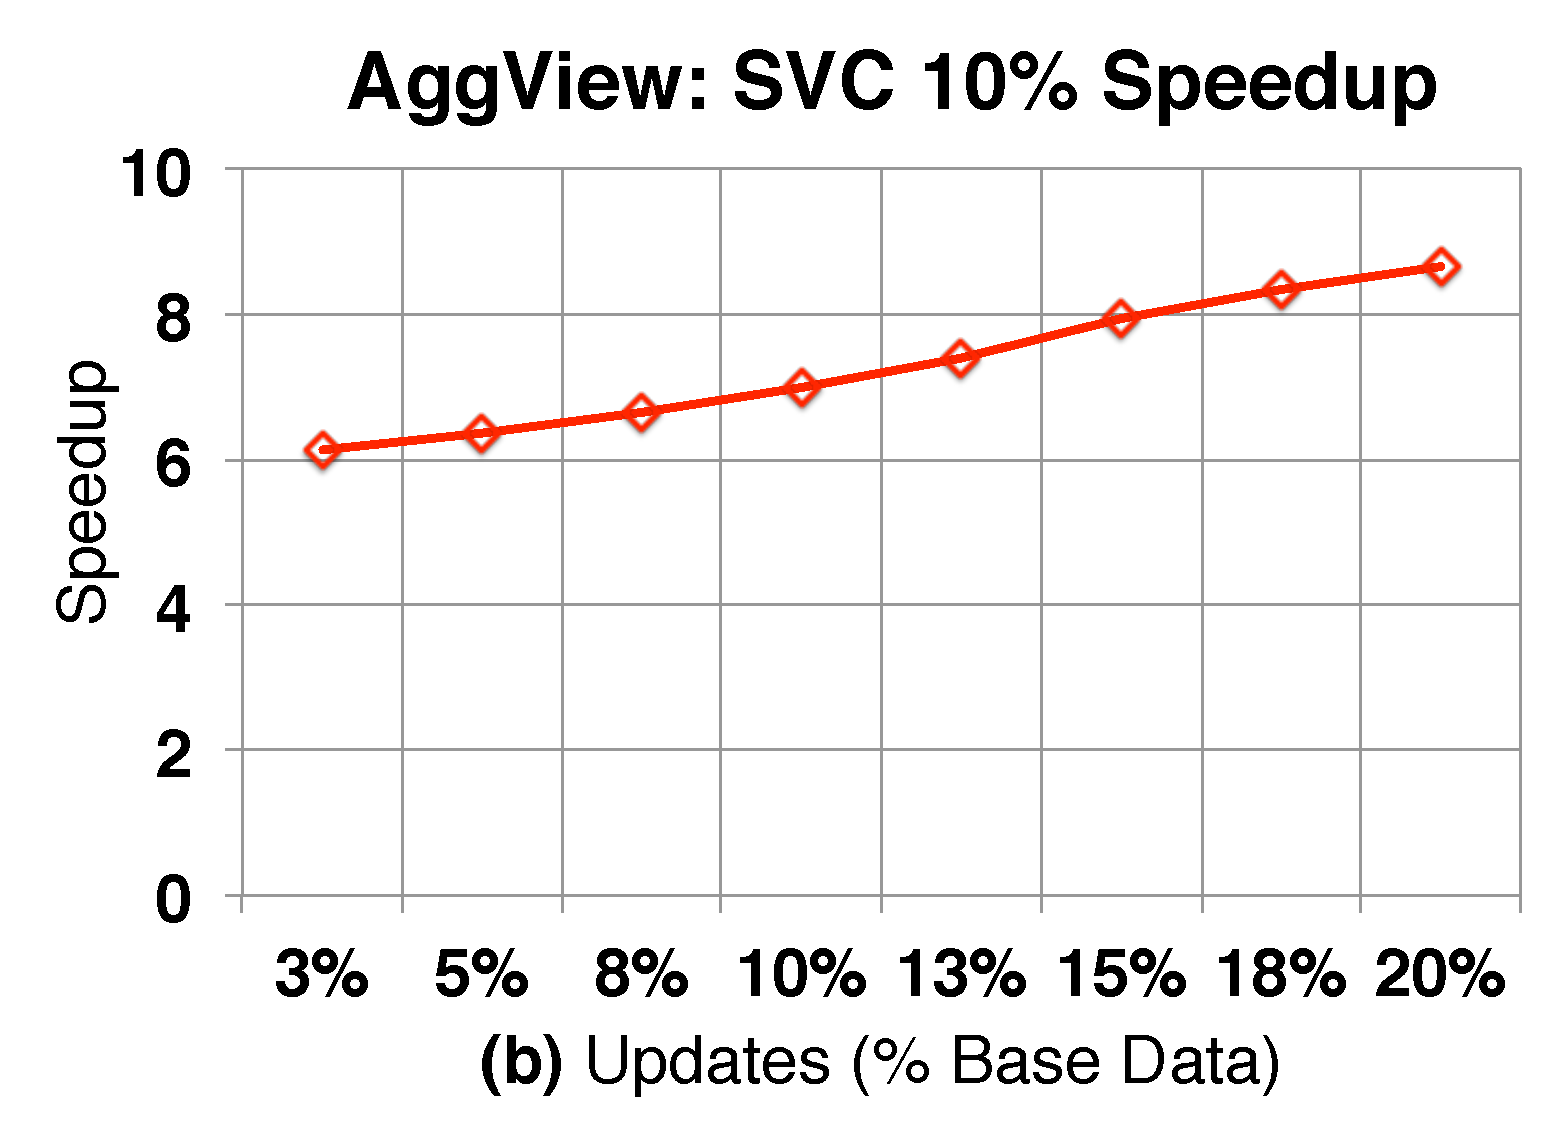
\includegraphics[scale=0.14]{exp/msdc_2.pdf}
  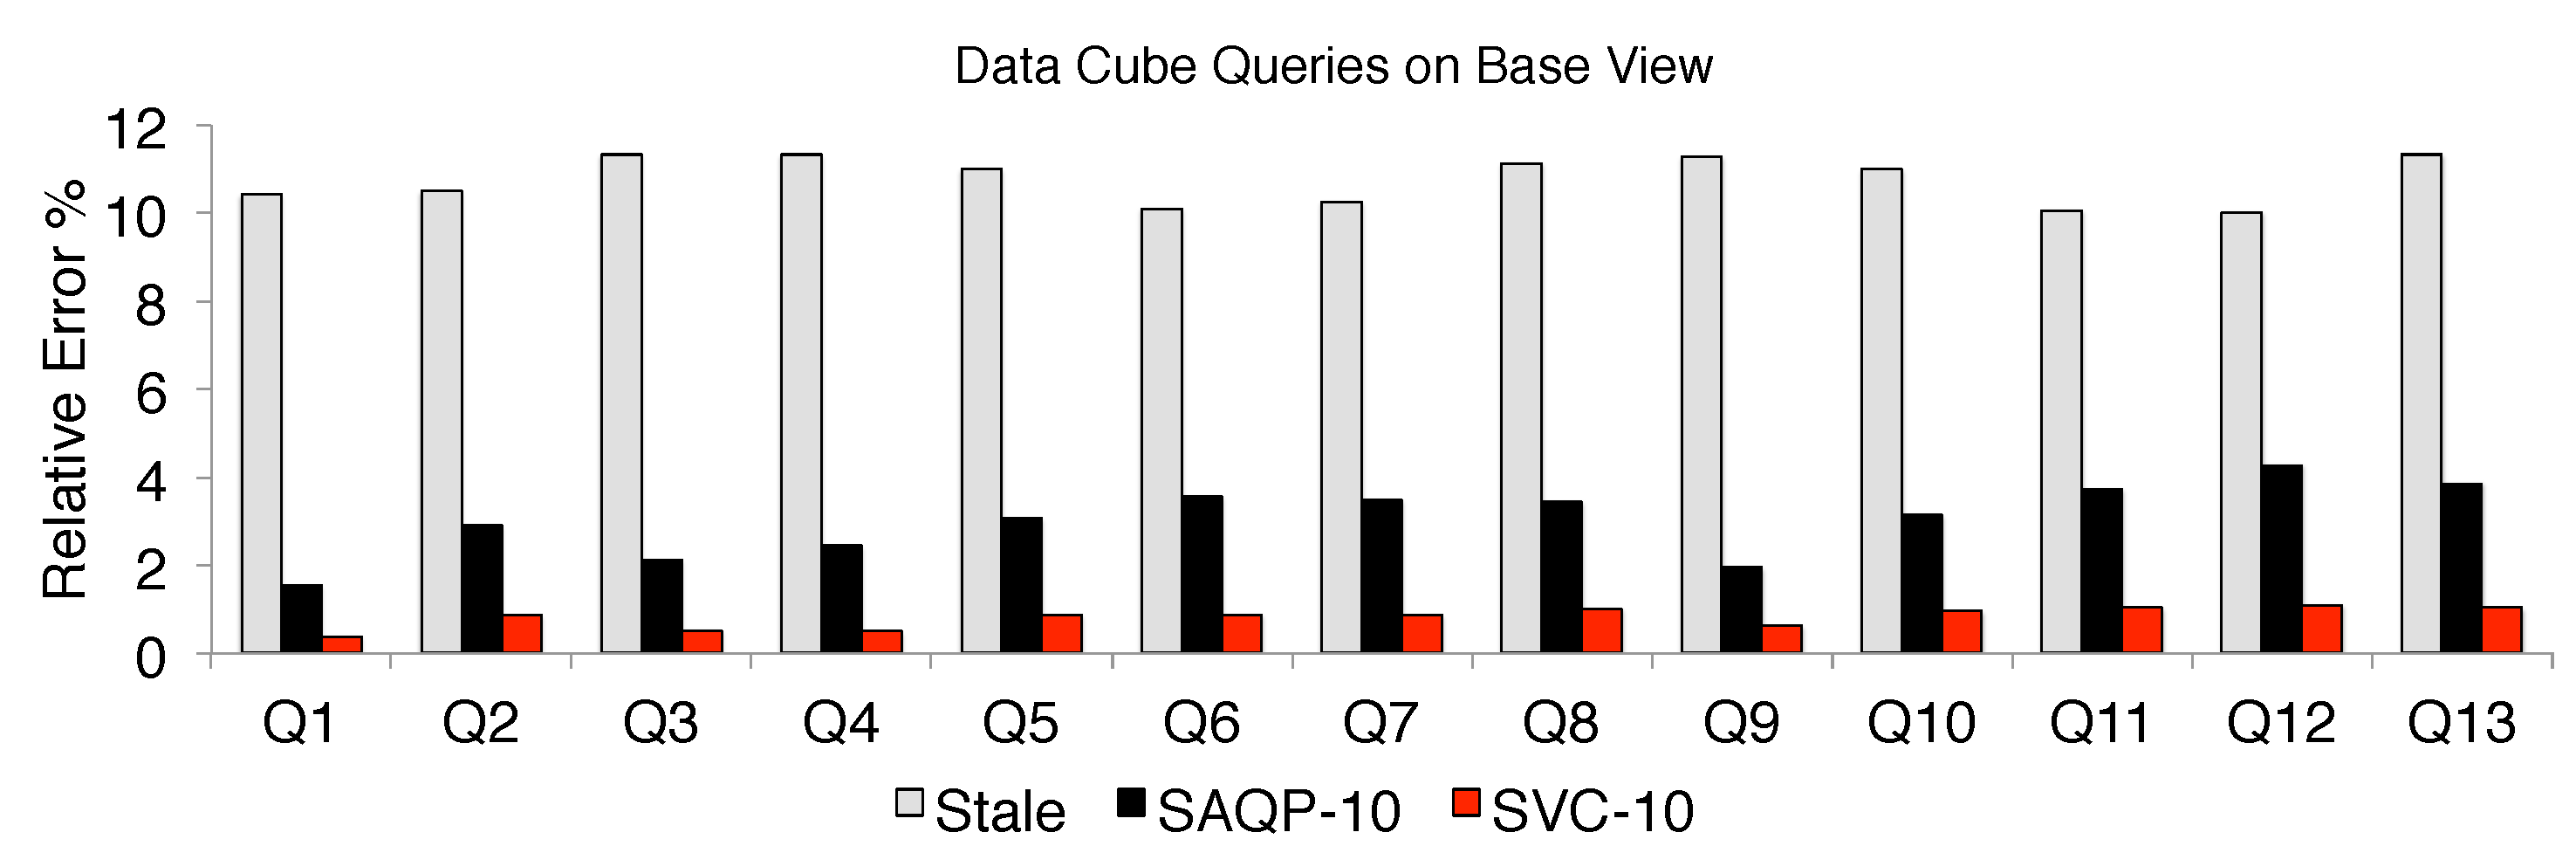
\includegraphics[scale=0.16]{exp/msdc_3.pdf}
  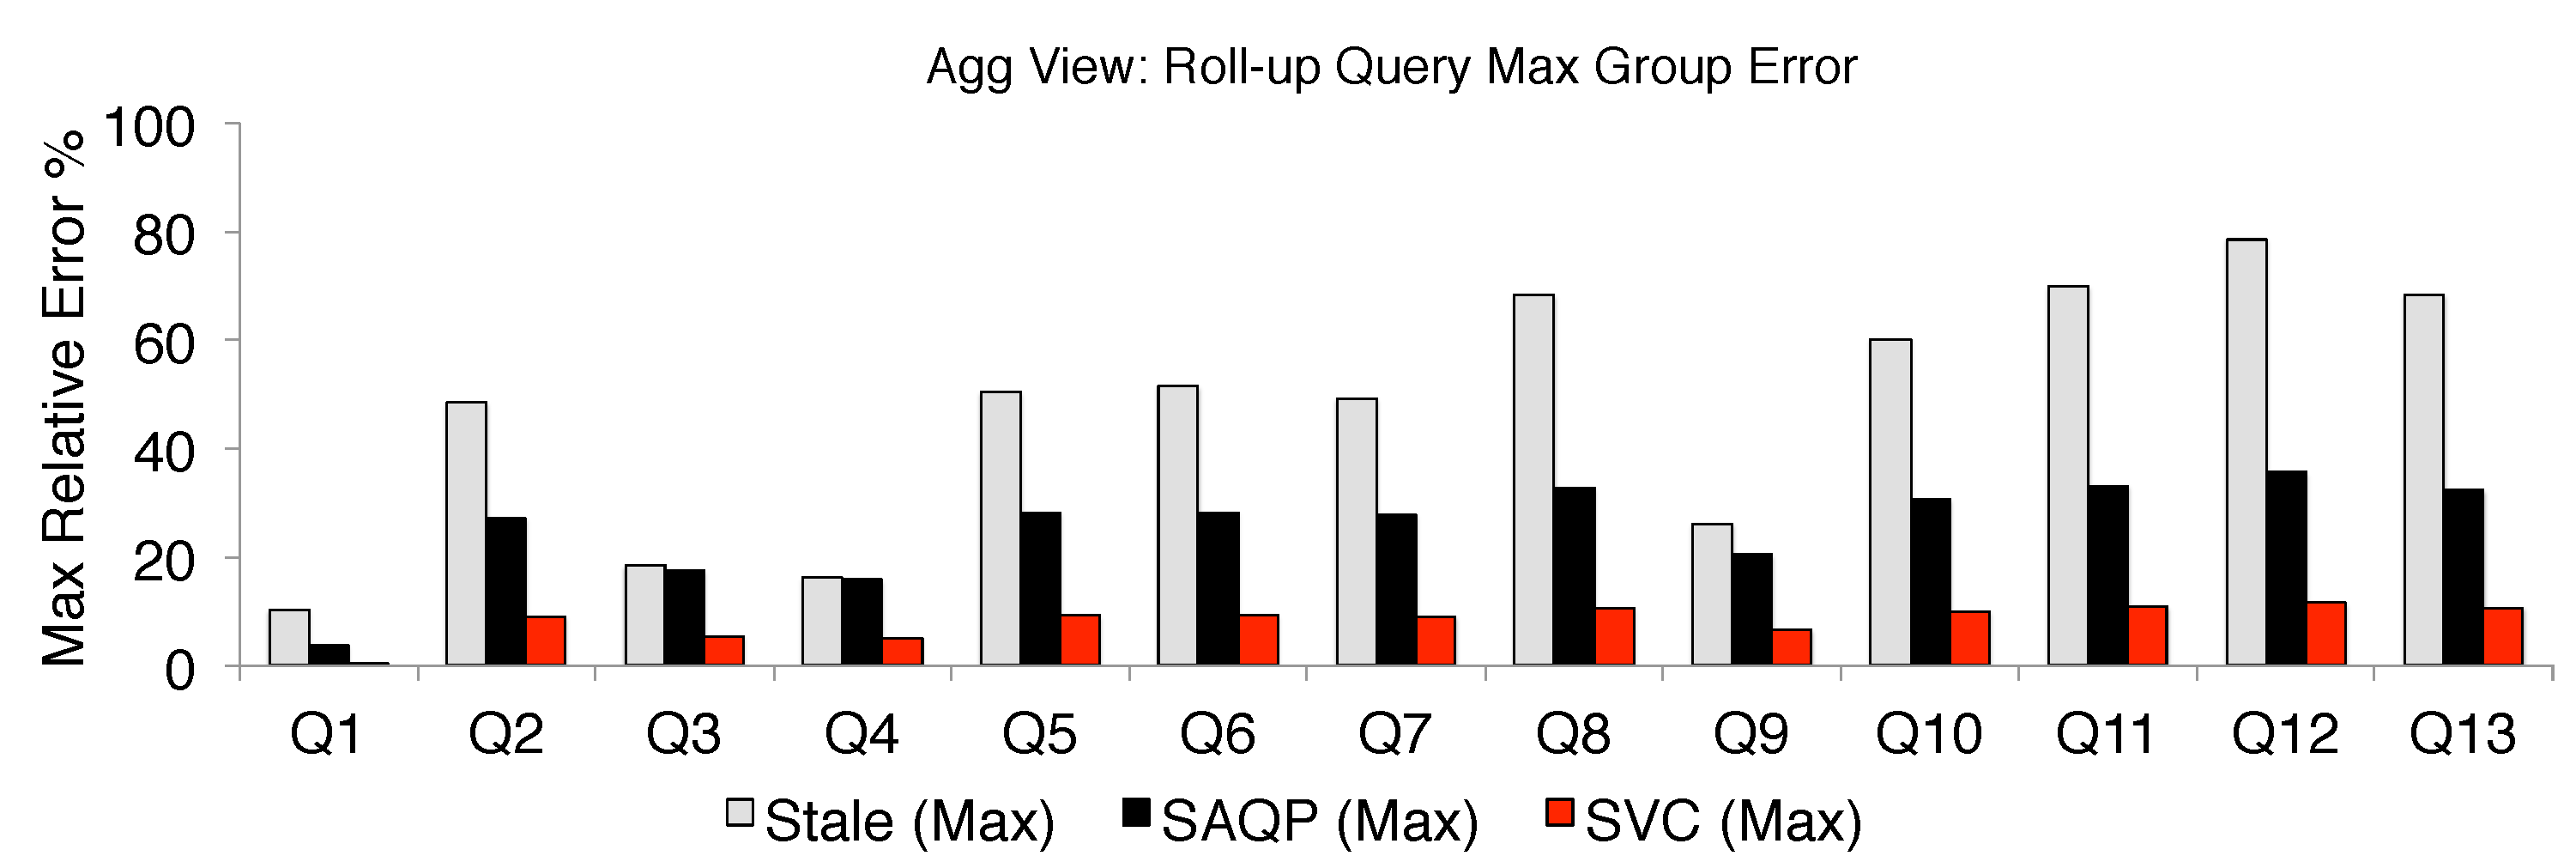
\includegraphics[scale=0.16]{exp/msdc_4.pdf}
  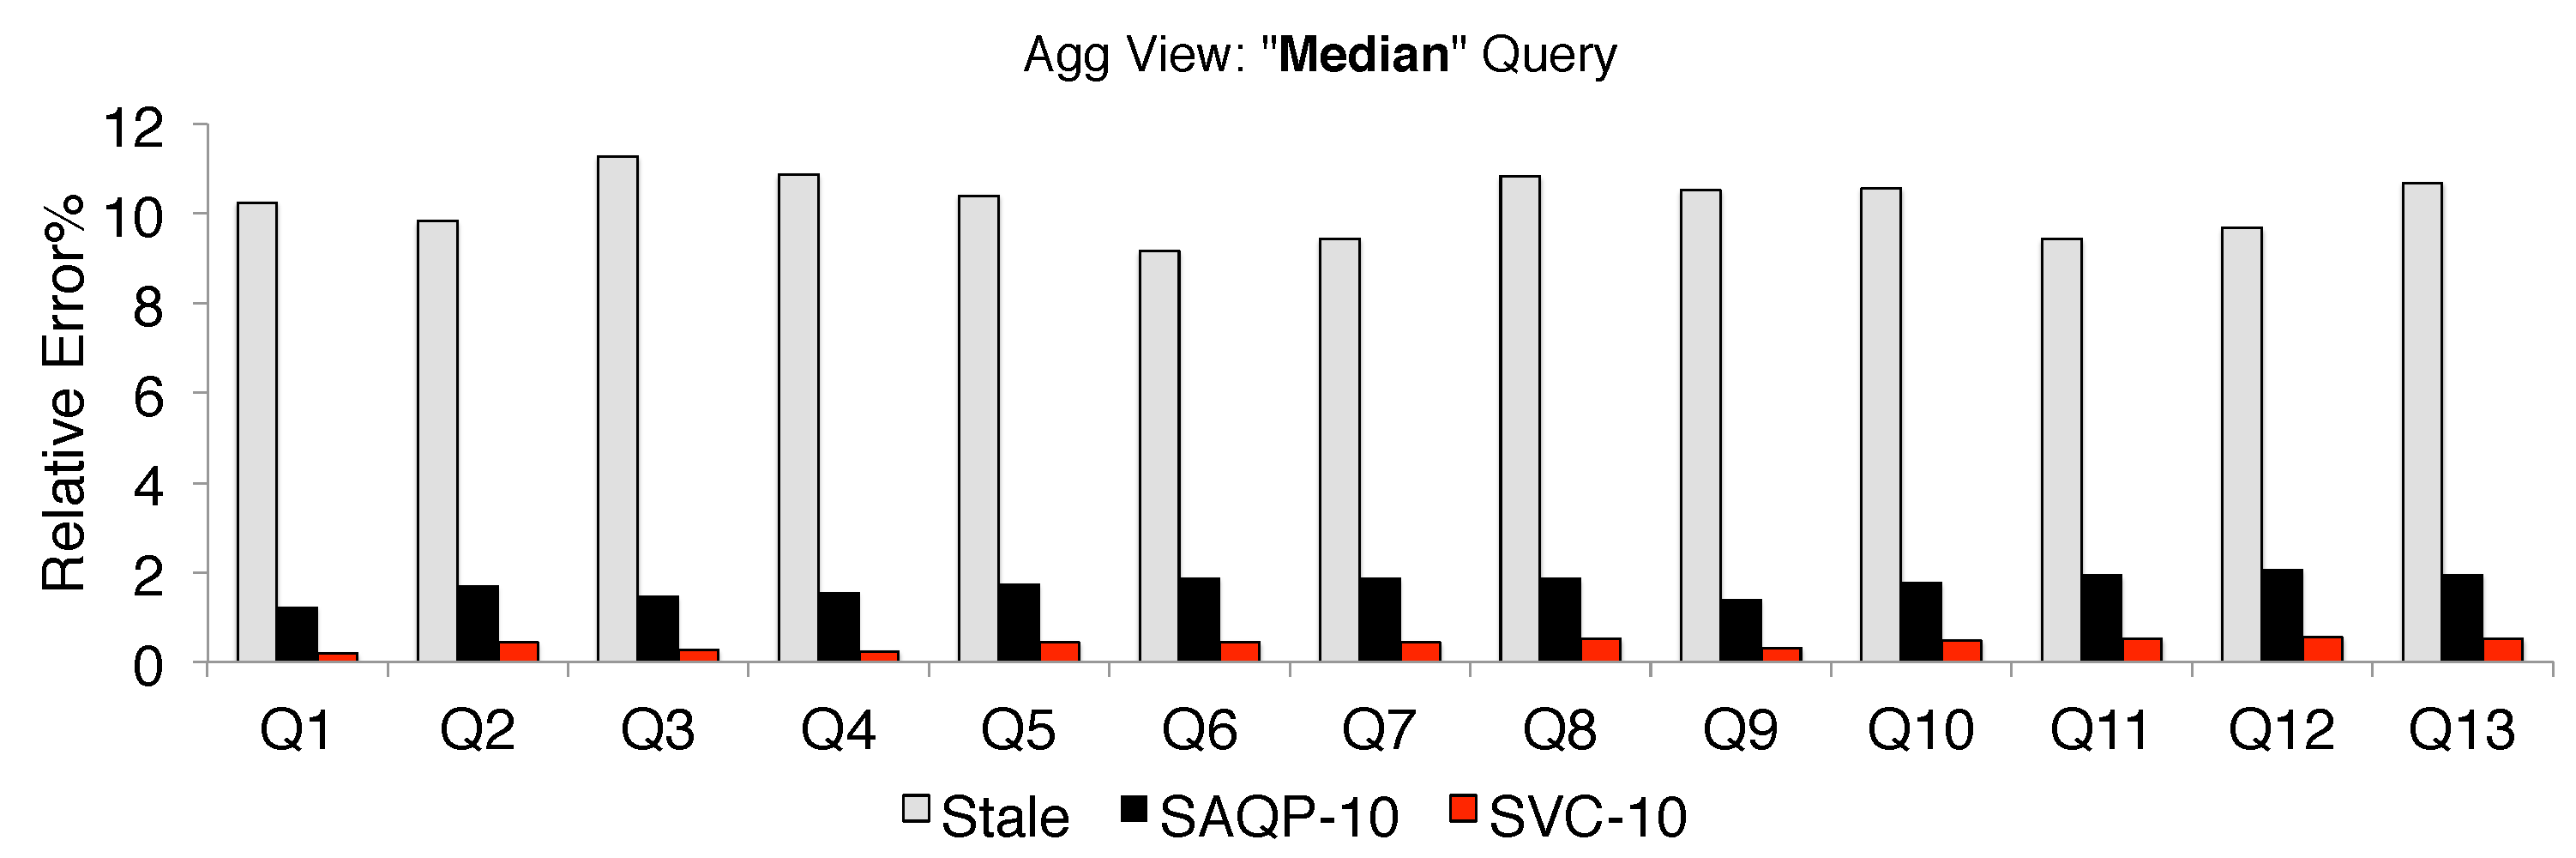
\includegraphics[scale=0.16]{exp/msdc_5.pdf}
  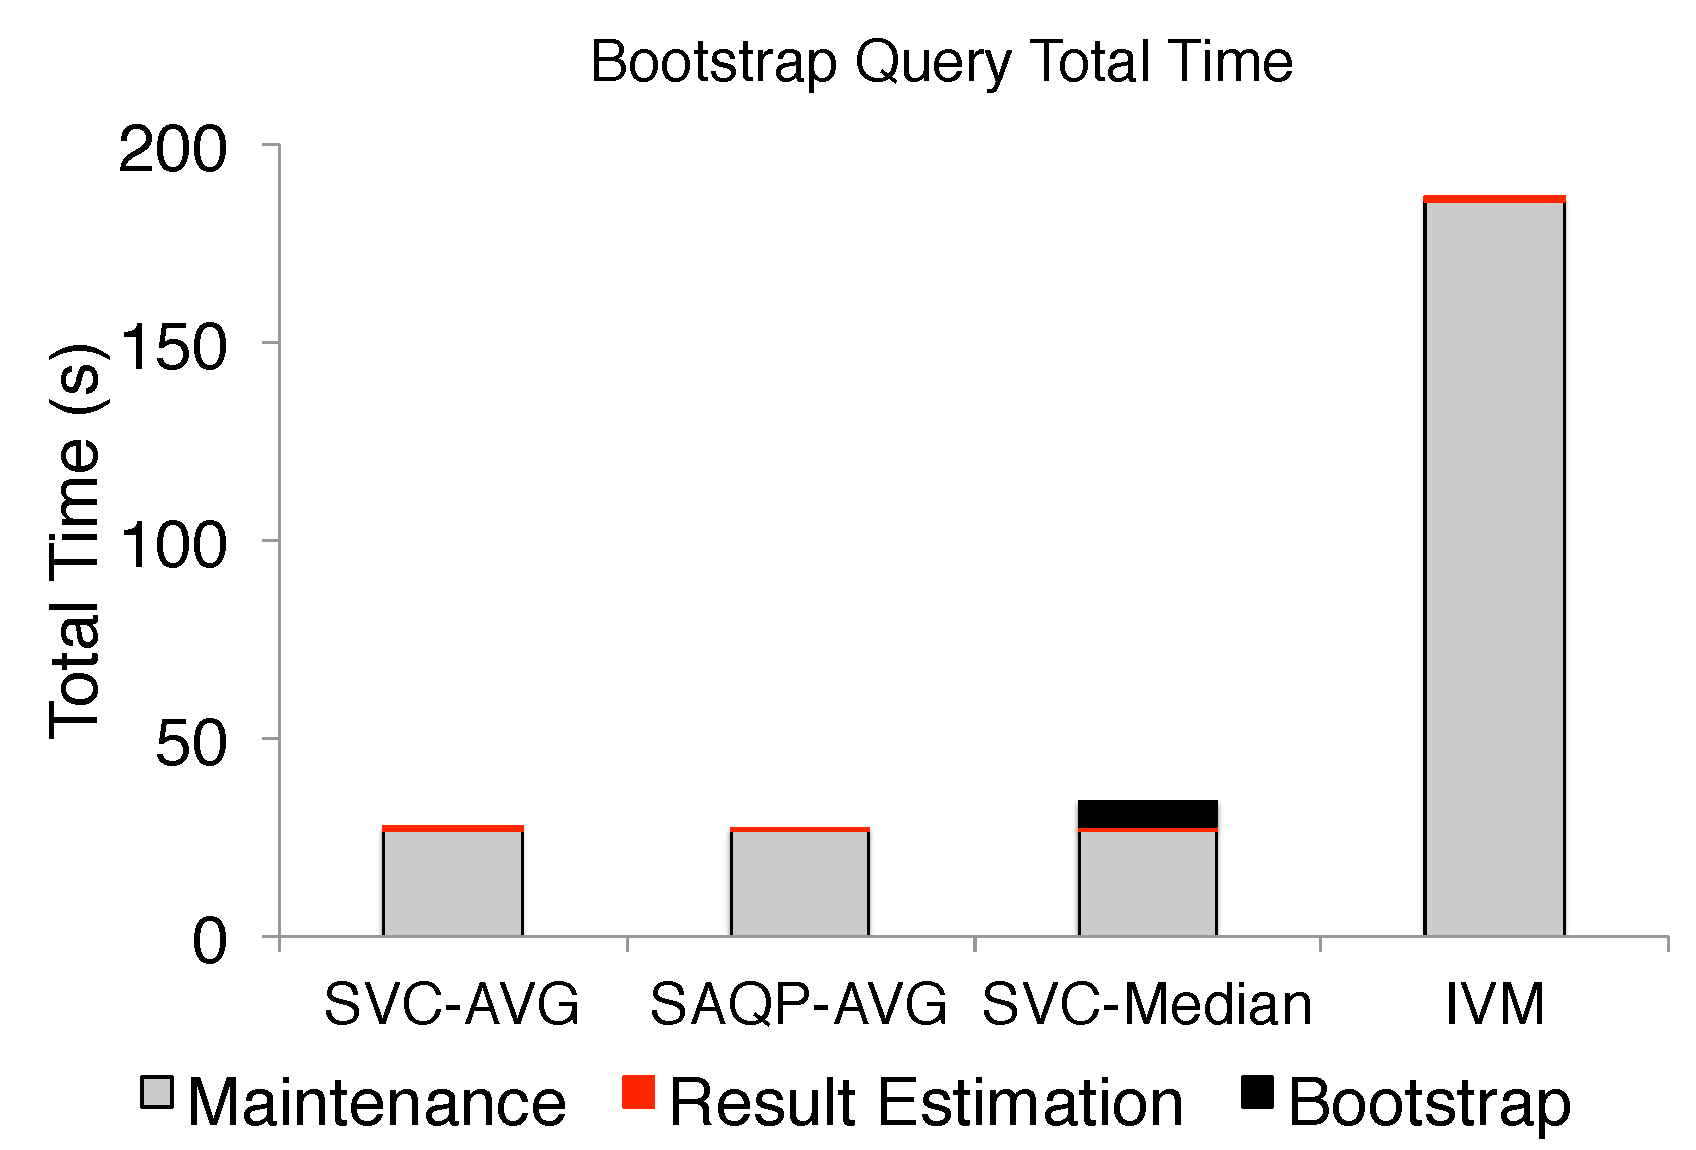
\includegraphics[scale=0.16]{exp/msdc_6.pdf}

 \caption{TODO}
\end{figure}

\subsubsection{TPCD Query Views}
\begin{figure}[t]
\centering
 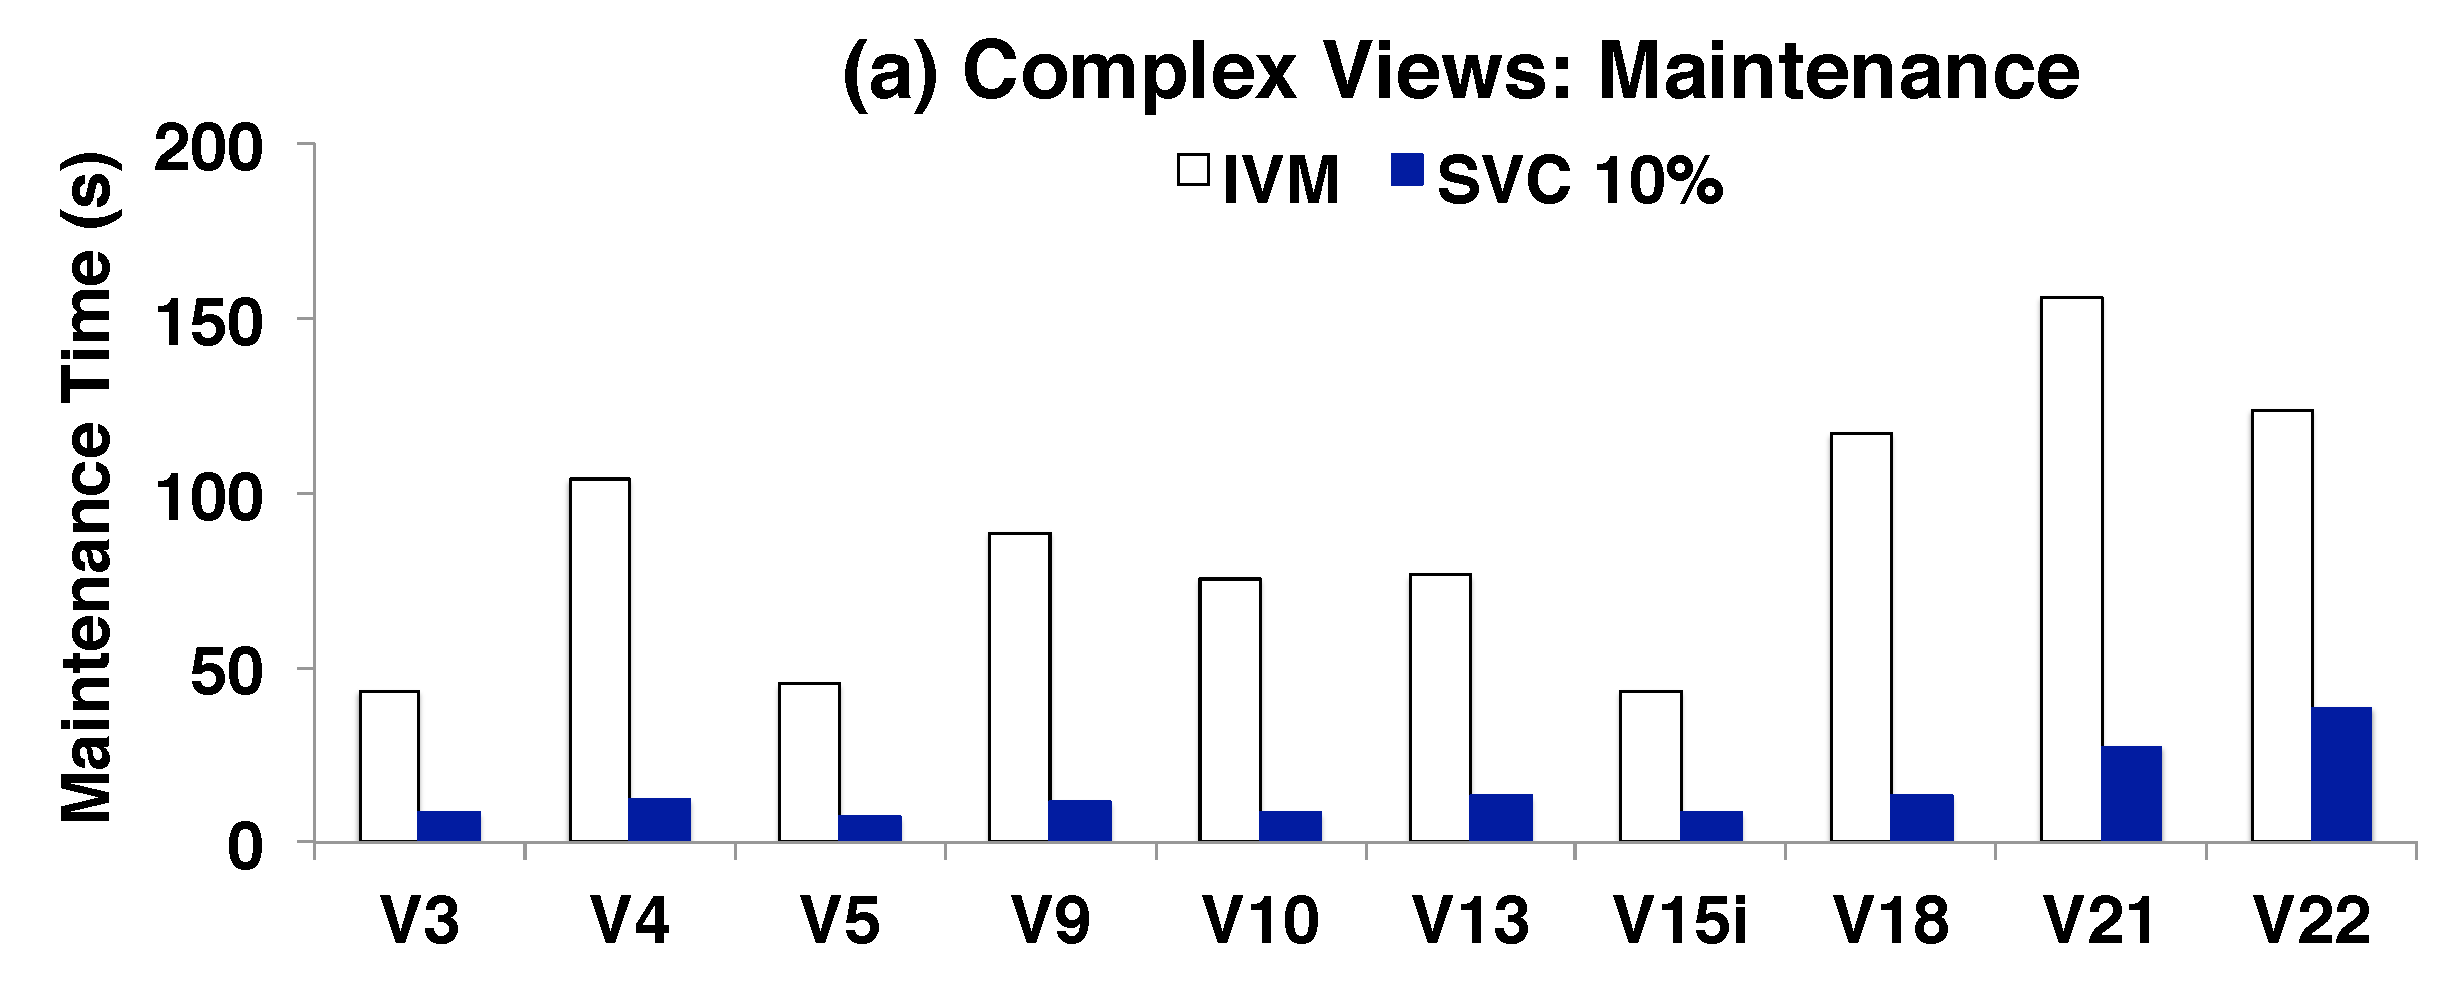
\includegraphics[scale=0.16]{exp/msqv_1.pdf}
 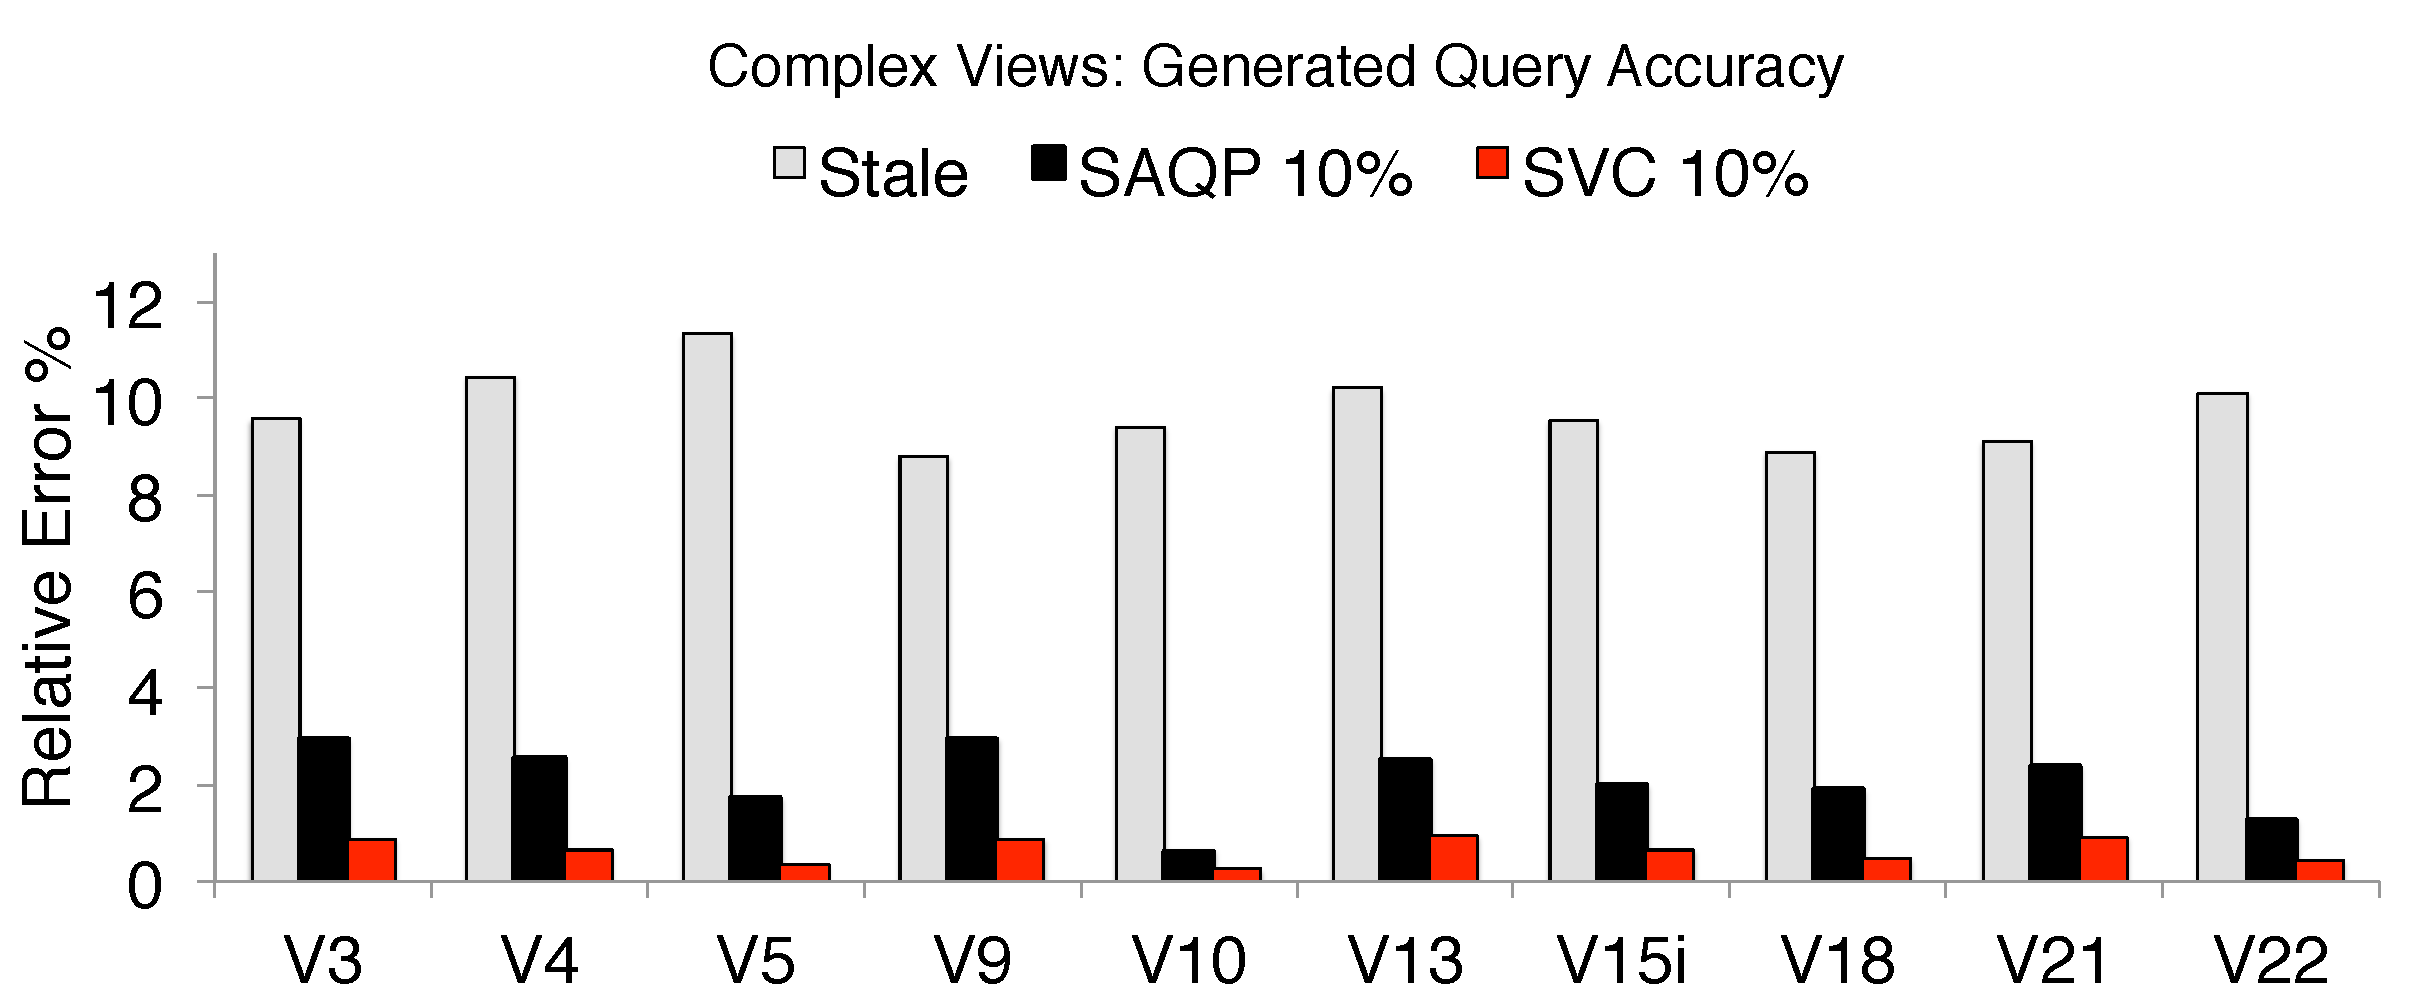
\includegraphics[scale=0.16]{exp/msqv_2.pdf}

 \caption{TODO}
\end{figure}

\subsection{Outlier Indexing}
\begin{figure}[t]
\centering
 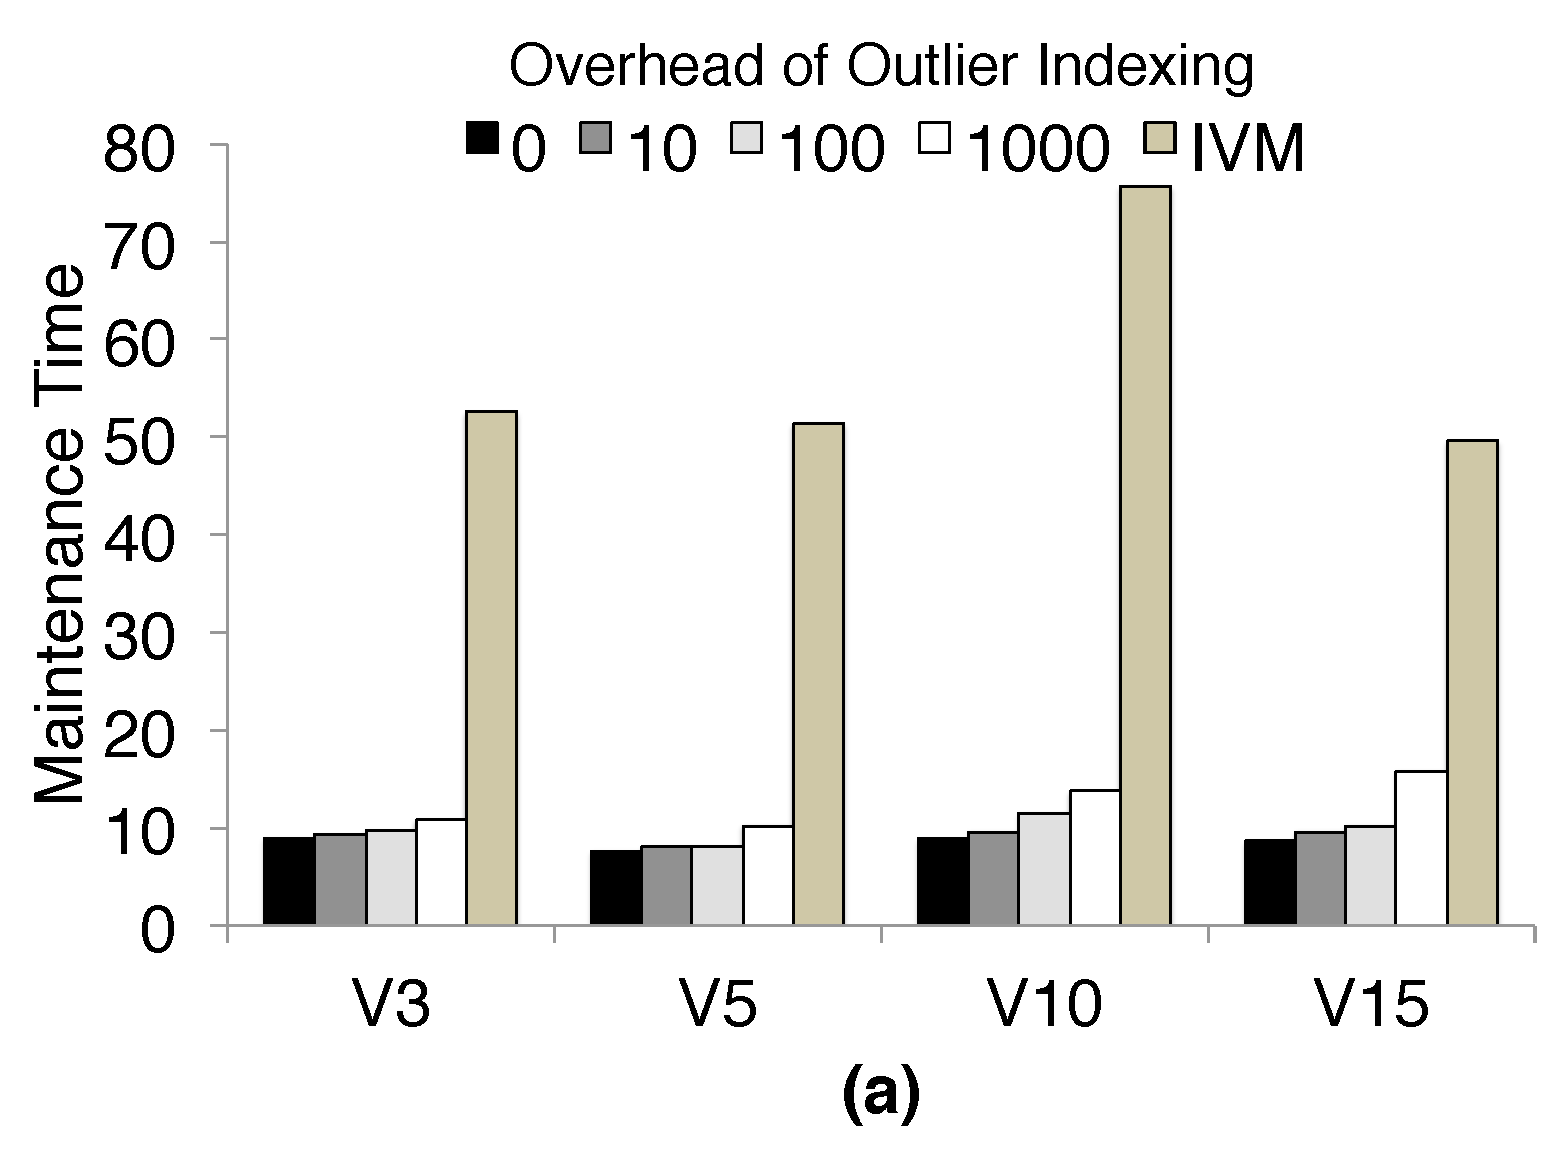
\includegraphics[scale=0.14]{exp/msoi_1.pdf}
 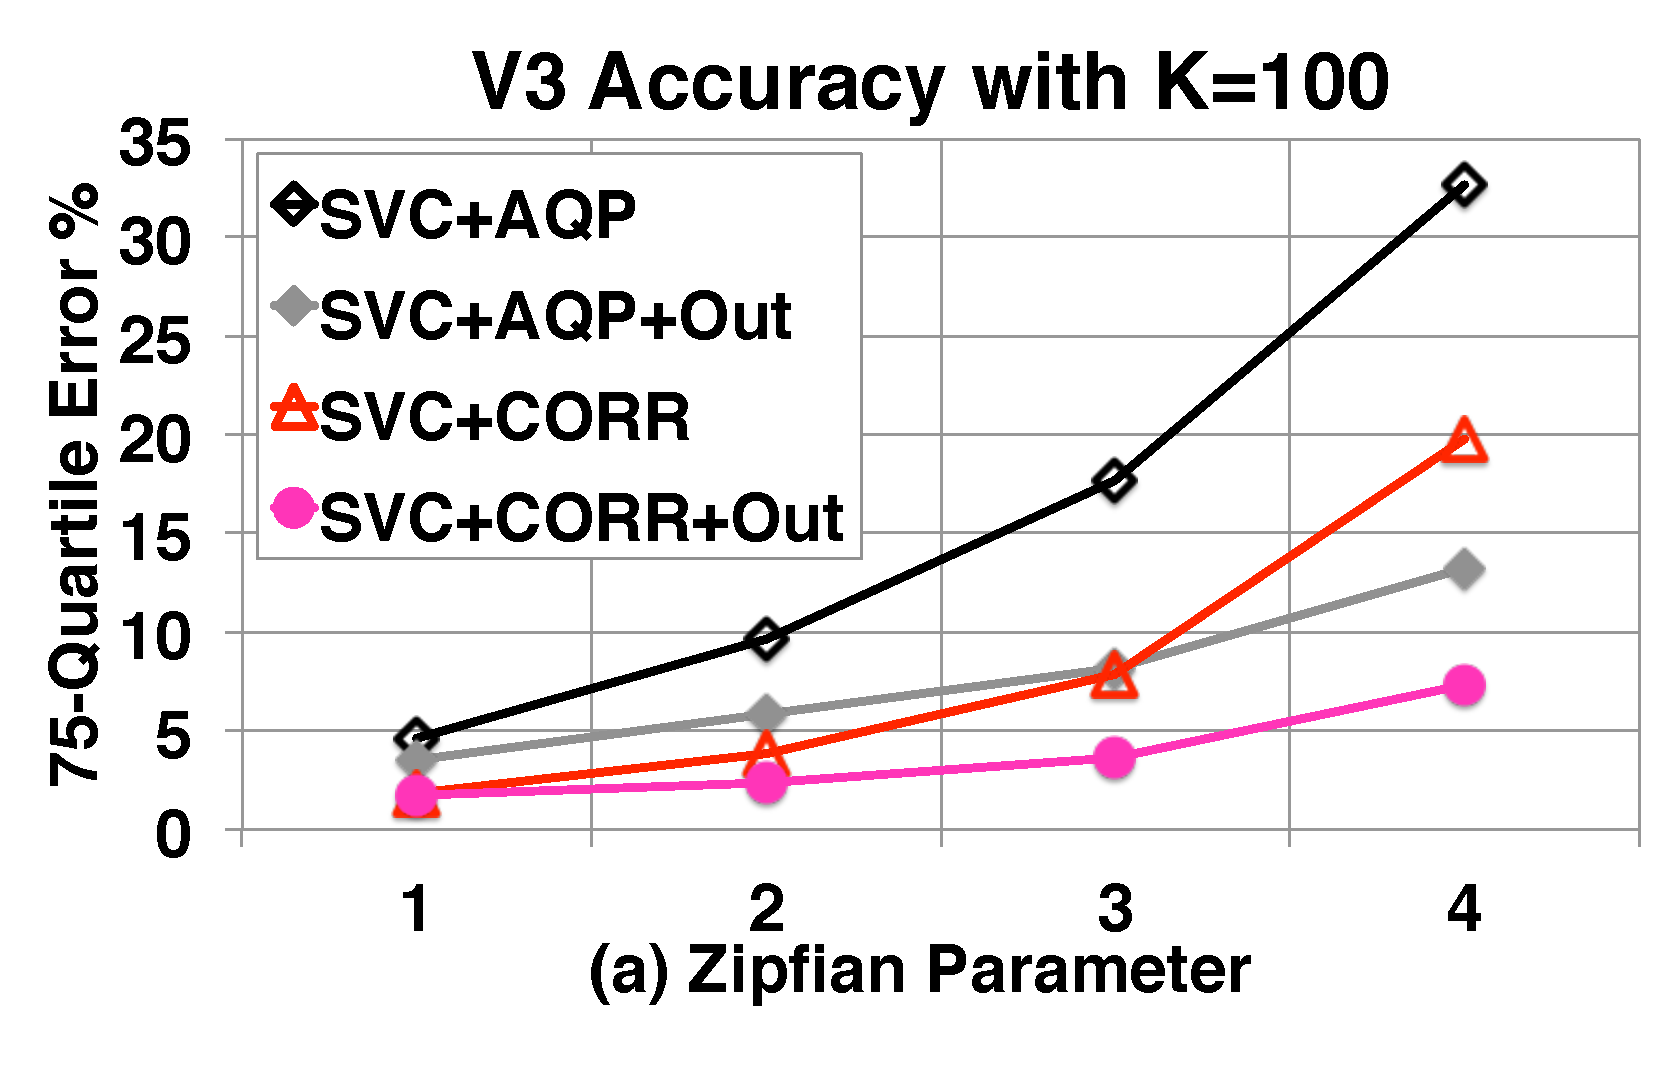
\includegraphics[scale=0.14]{exp/msoi_2.pdf}

 \caption{TODO}
\end{figure}

\subsection{Systems Considerations}
\begin{figure}[t]
\centering
 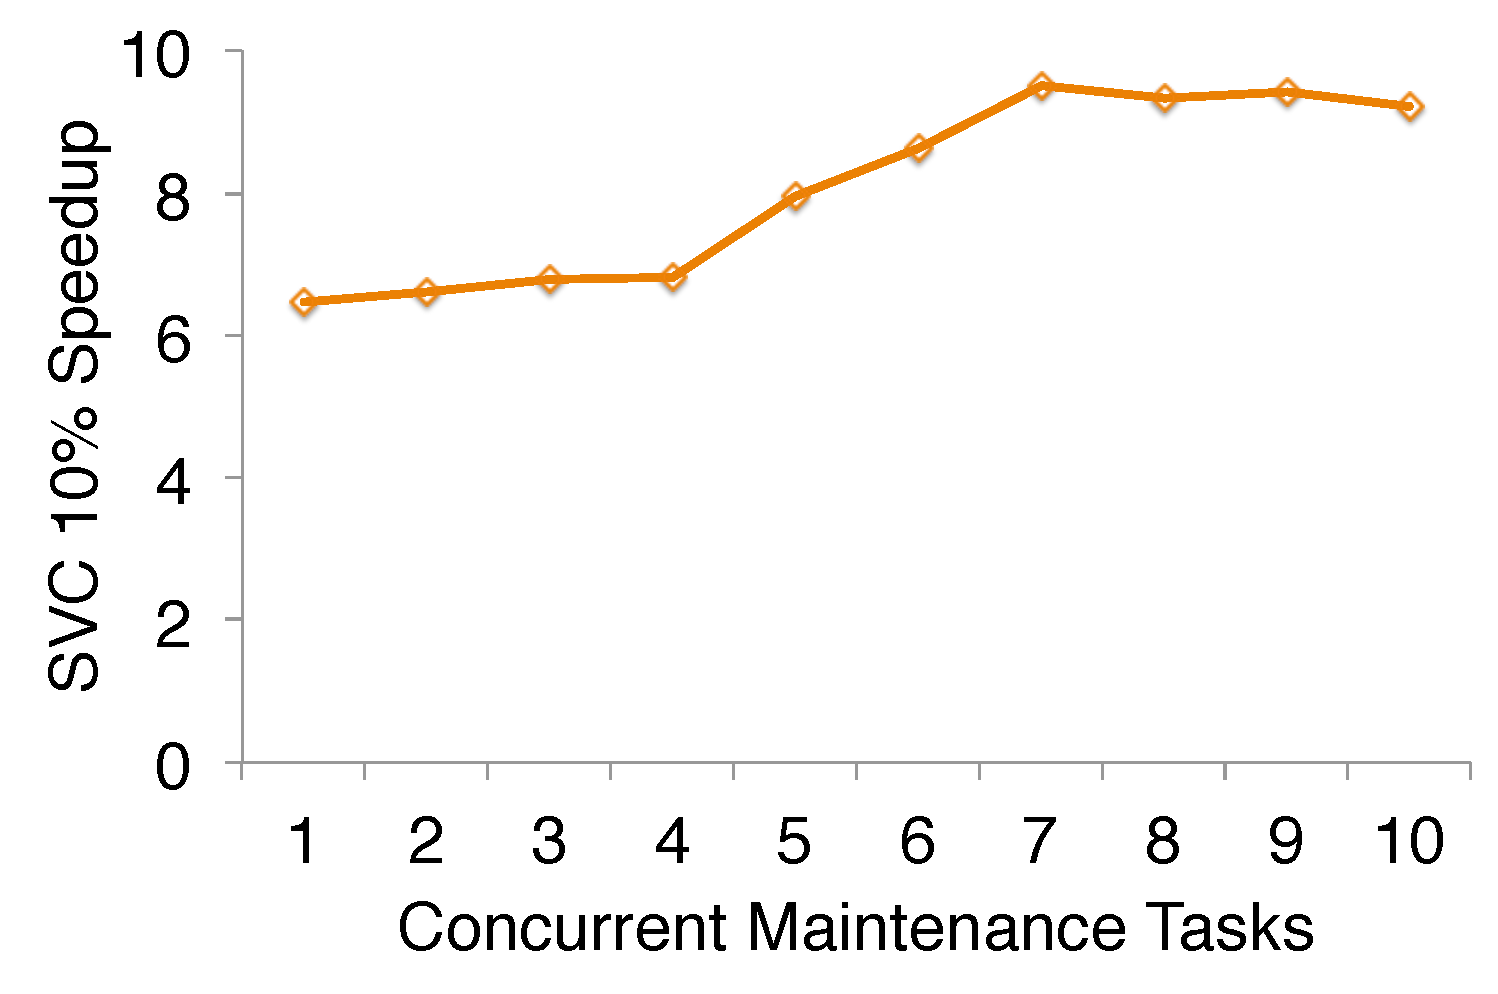
\includegraphics[scale=0.14]{exp/mssd_1.pdf}
 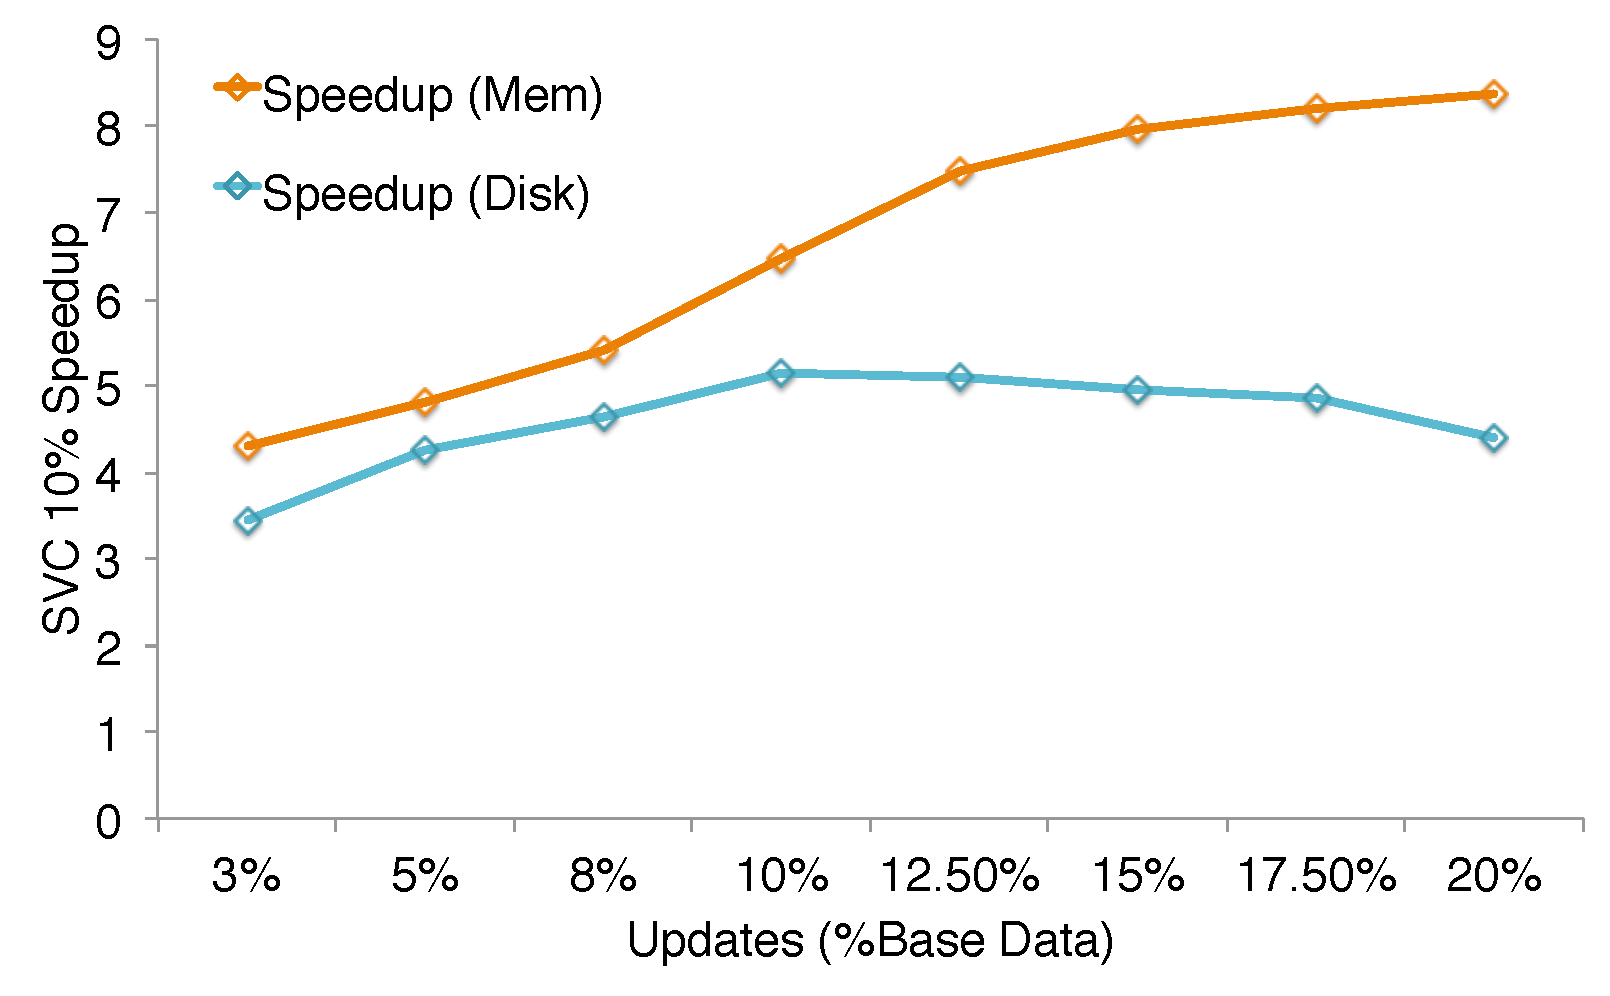
\includegraphics[scale=0.14]{exp/mssd_2.pdf}

 \caption{TODO}
\end{figure}

\subsection{Conviva}
\begin{figure}[t]
\centering
 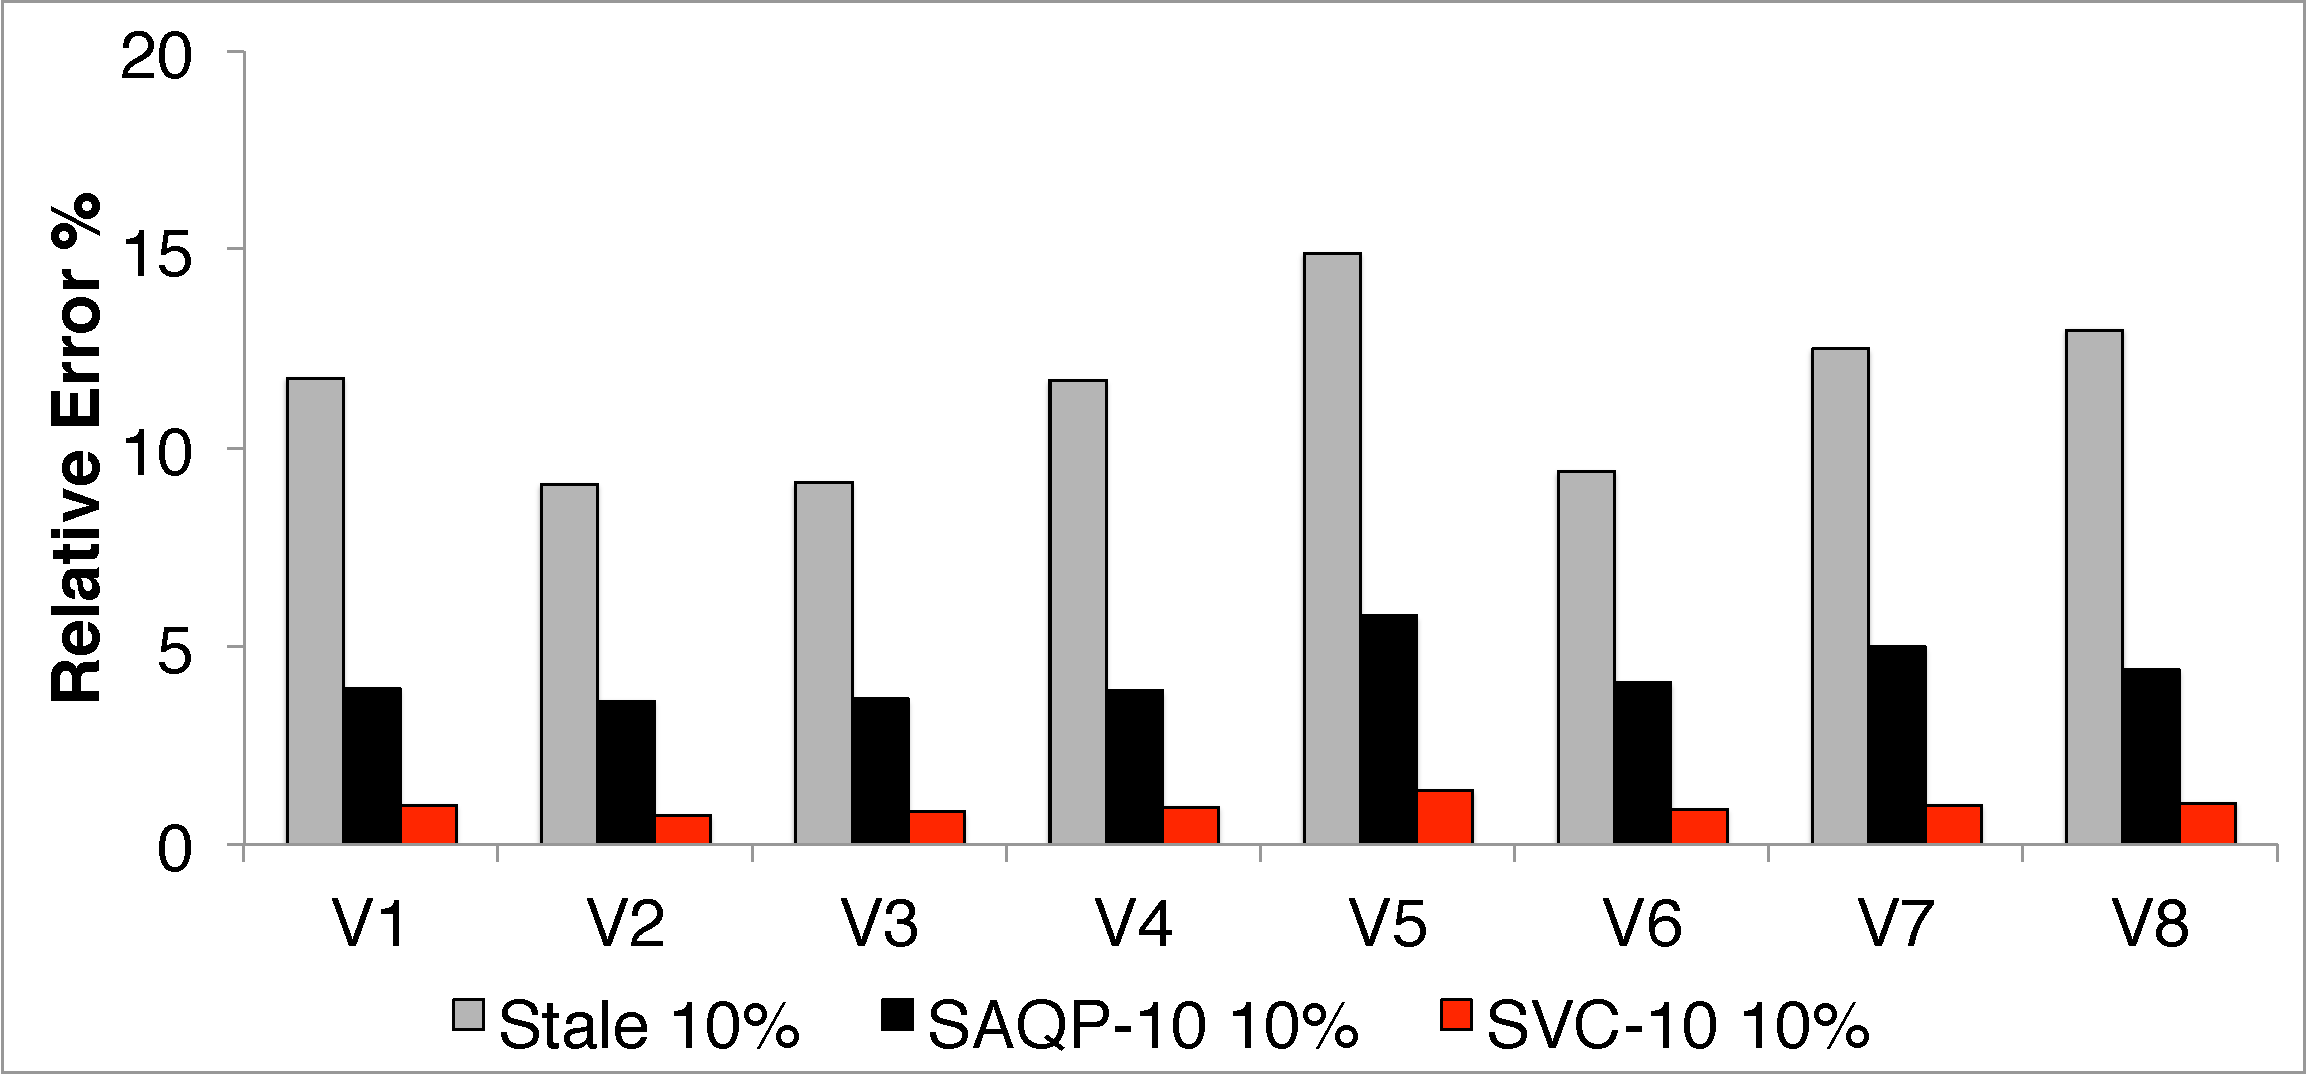
\includegraphics[scale=0.14]{exp/con_1.pdf}
 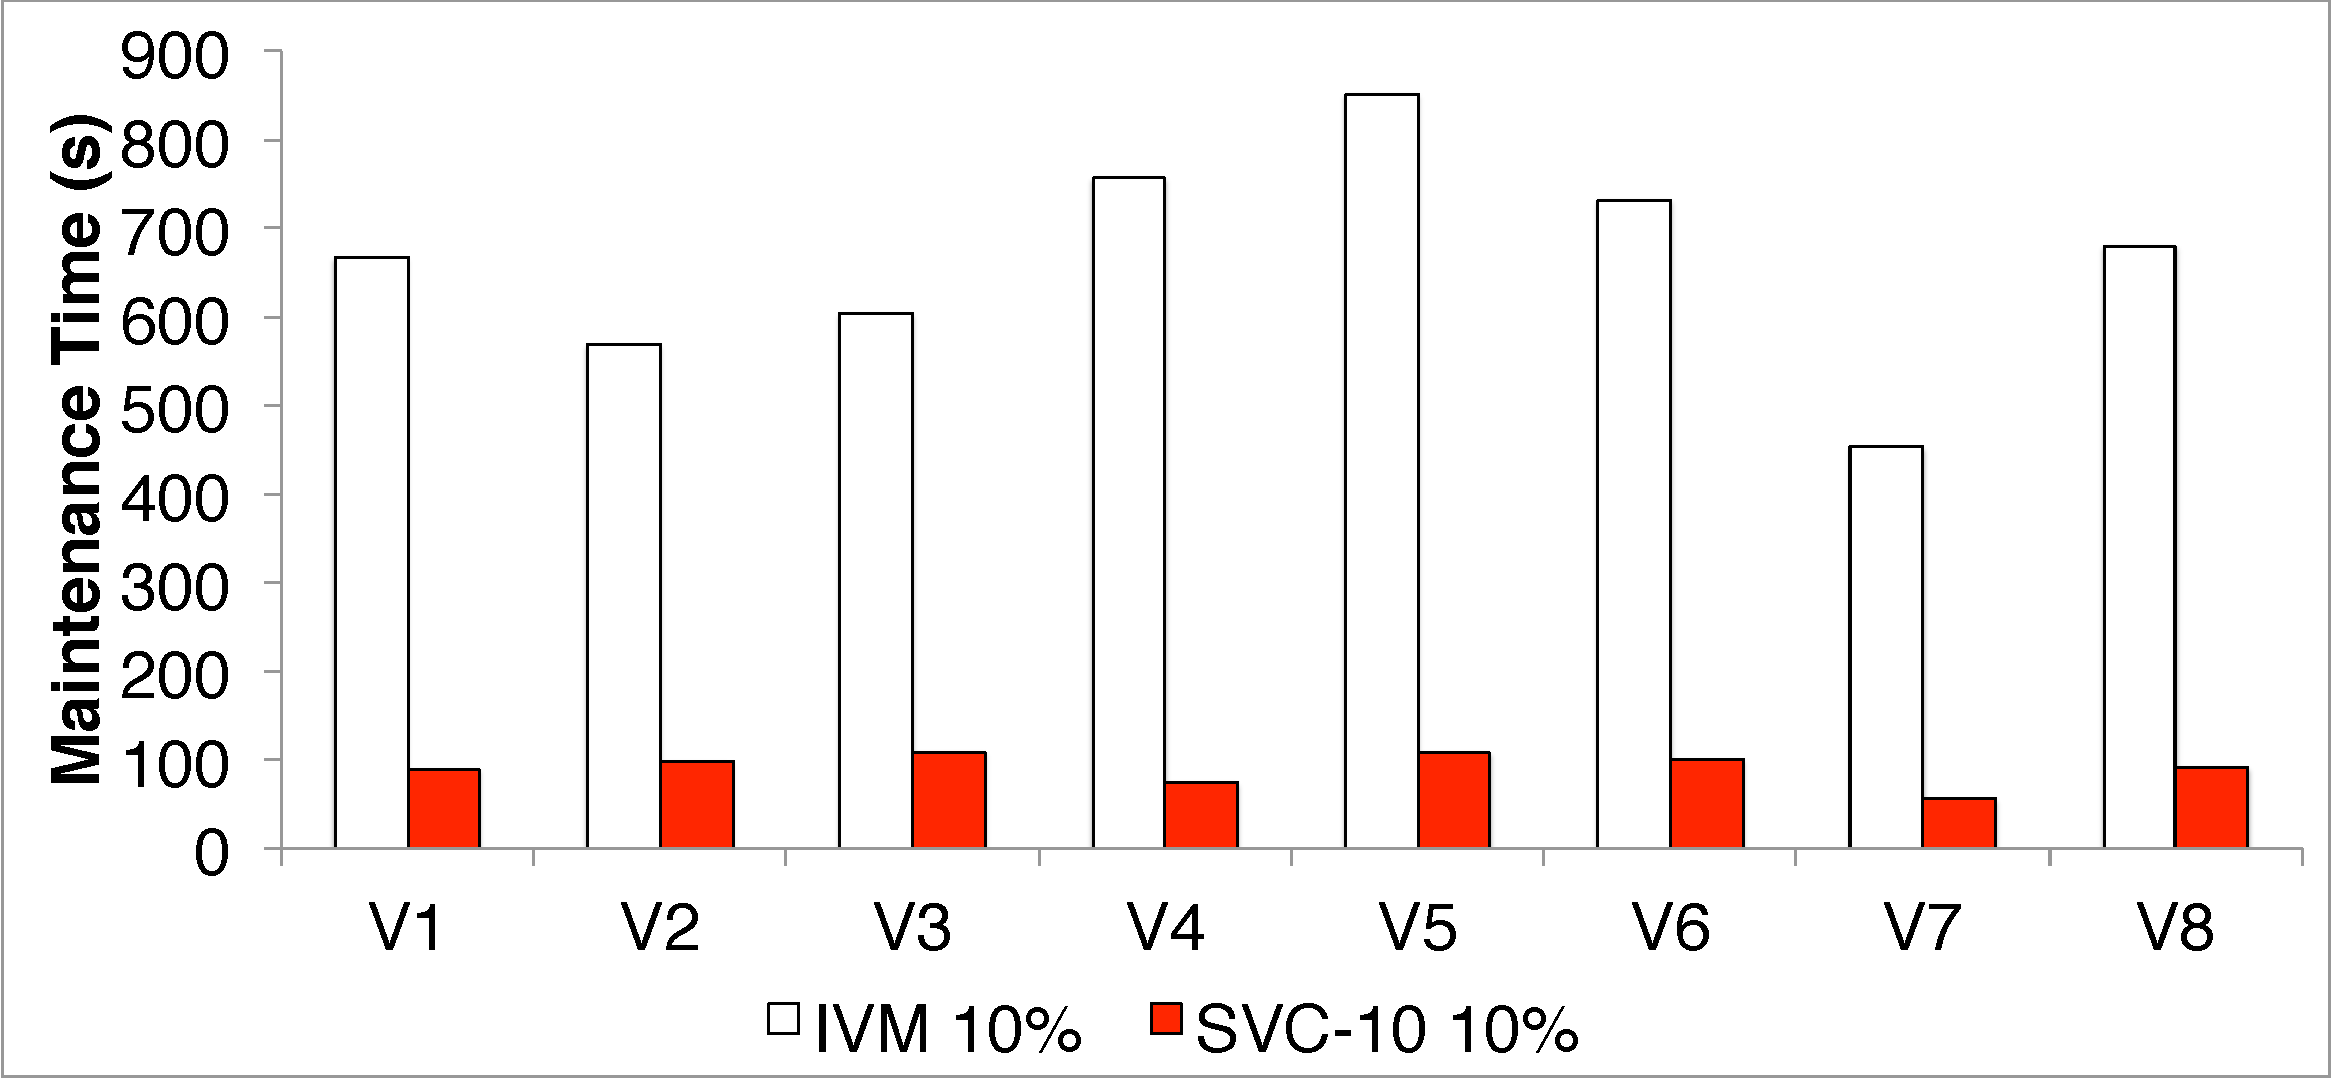
\includegraphics[scale=0.14]{exp/con_2.pdf}
 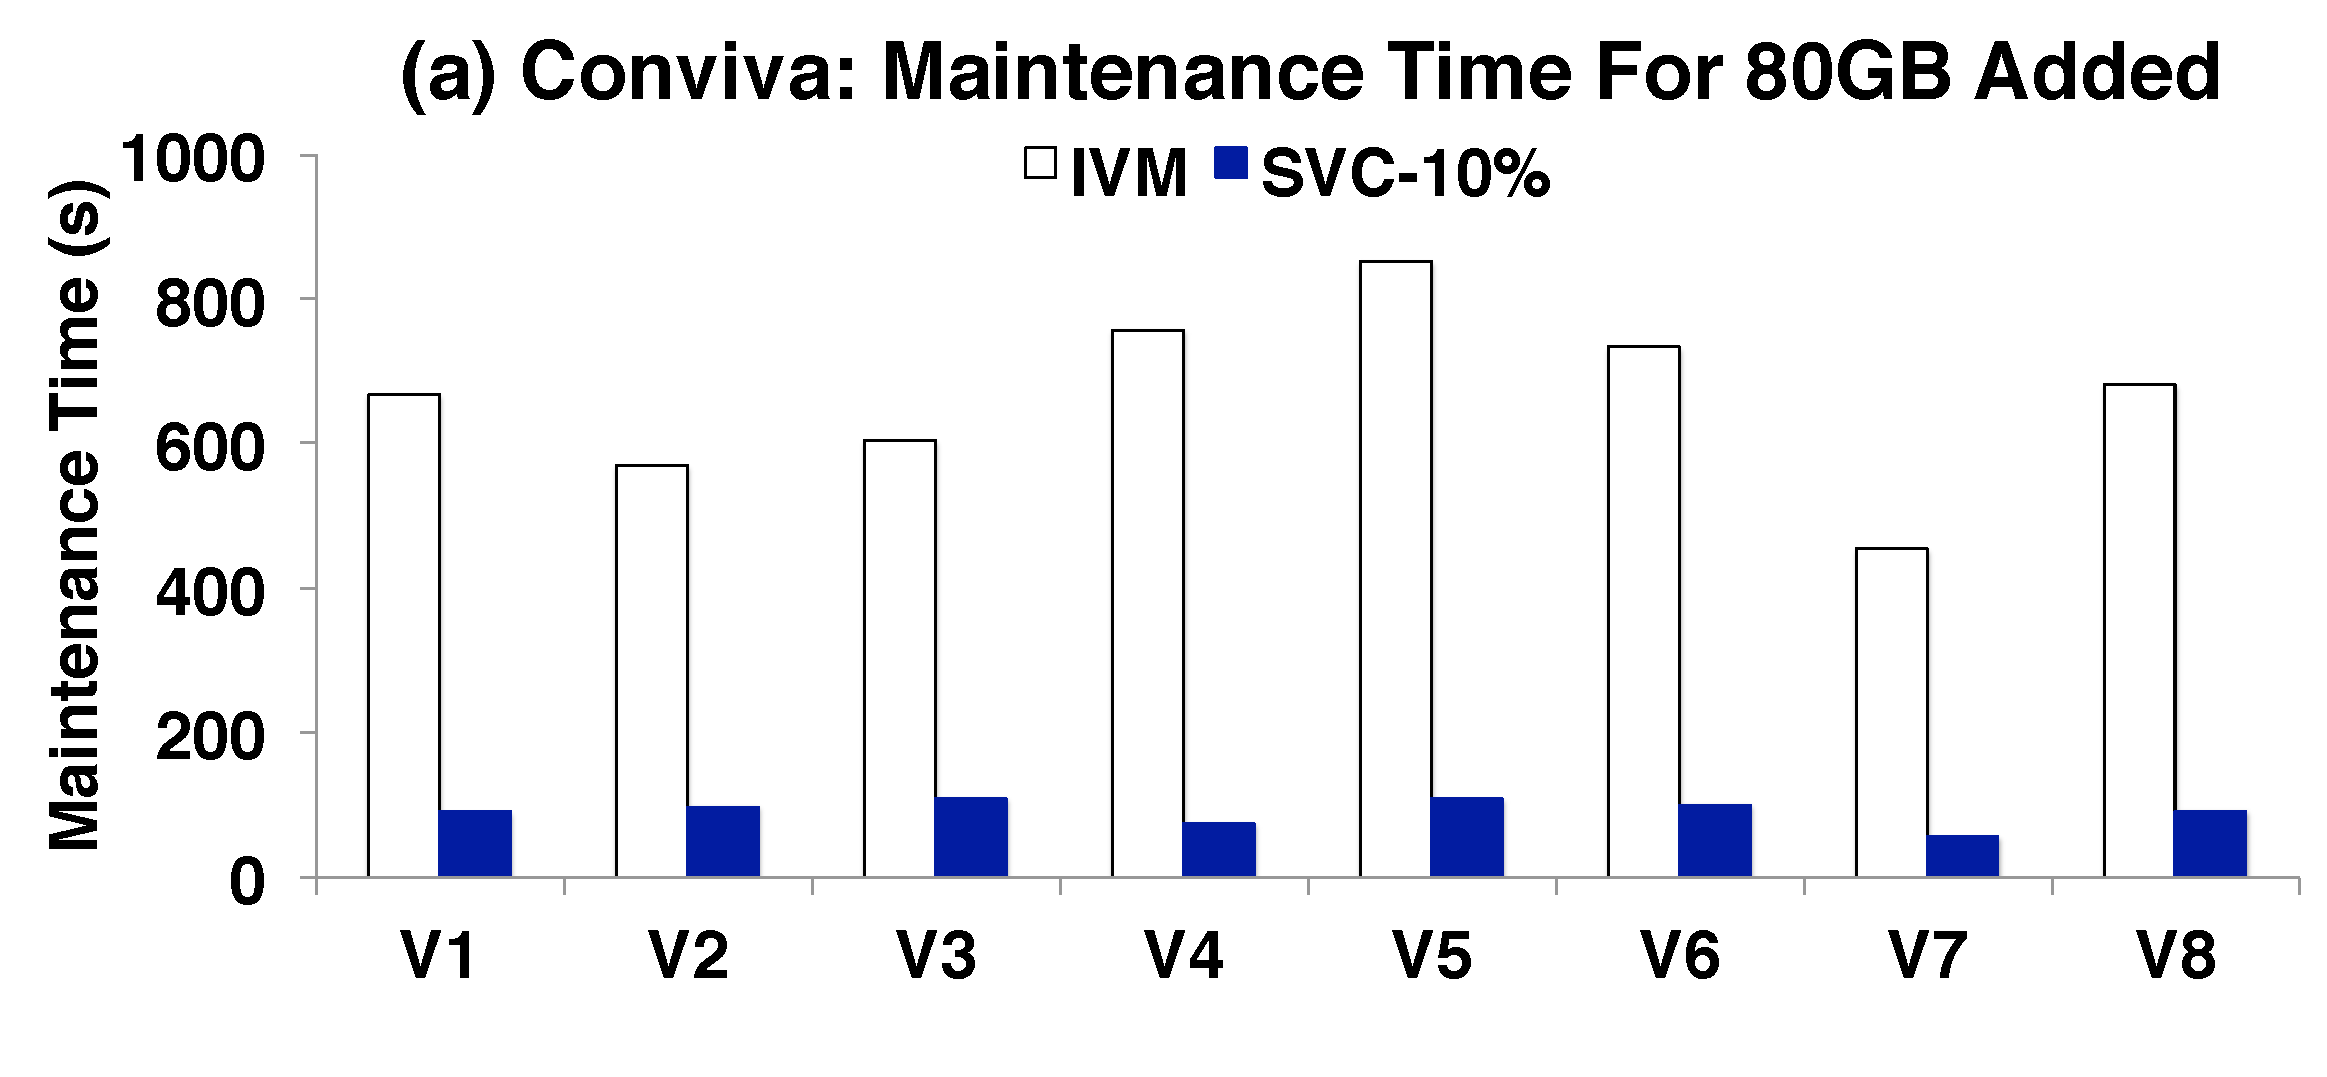
\includegraphics[scale=0.14]{exp/con_3.pdf}
 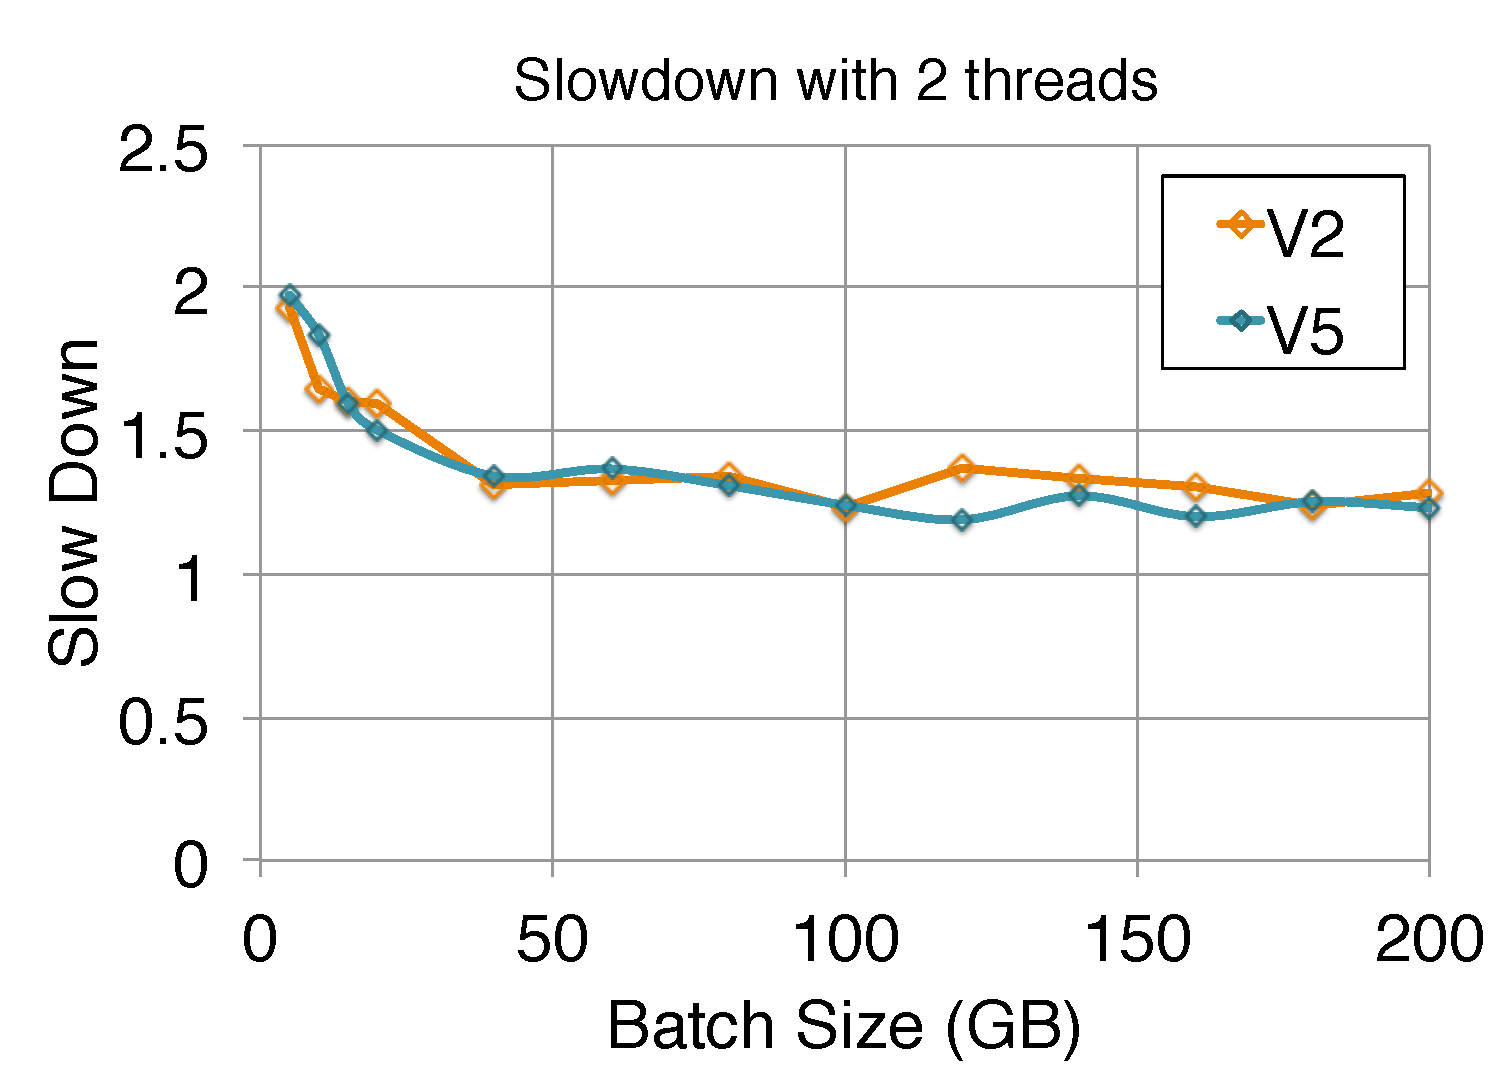
\includegraphics[scale=0.14]{exp/con_4.pdf}
 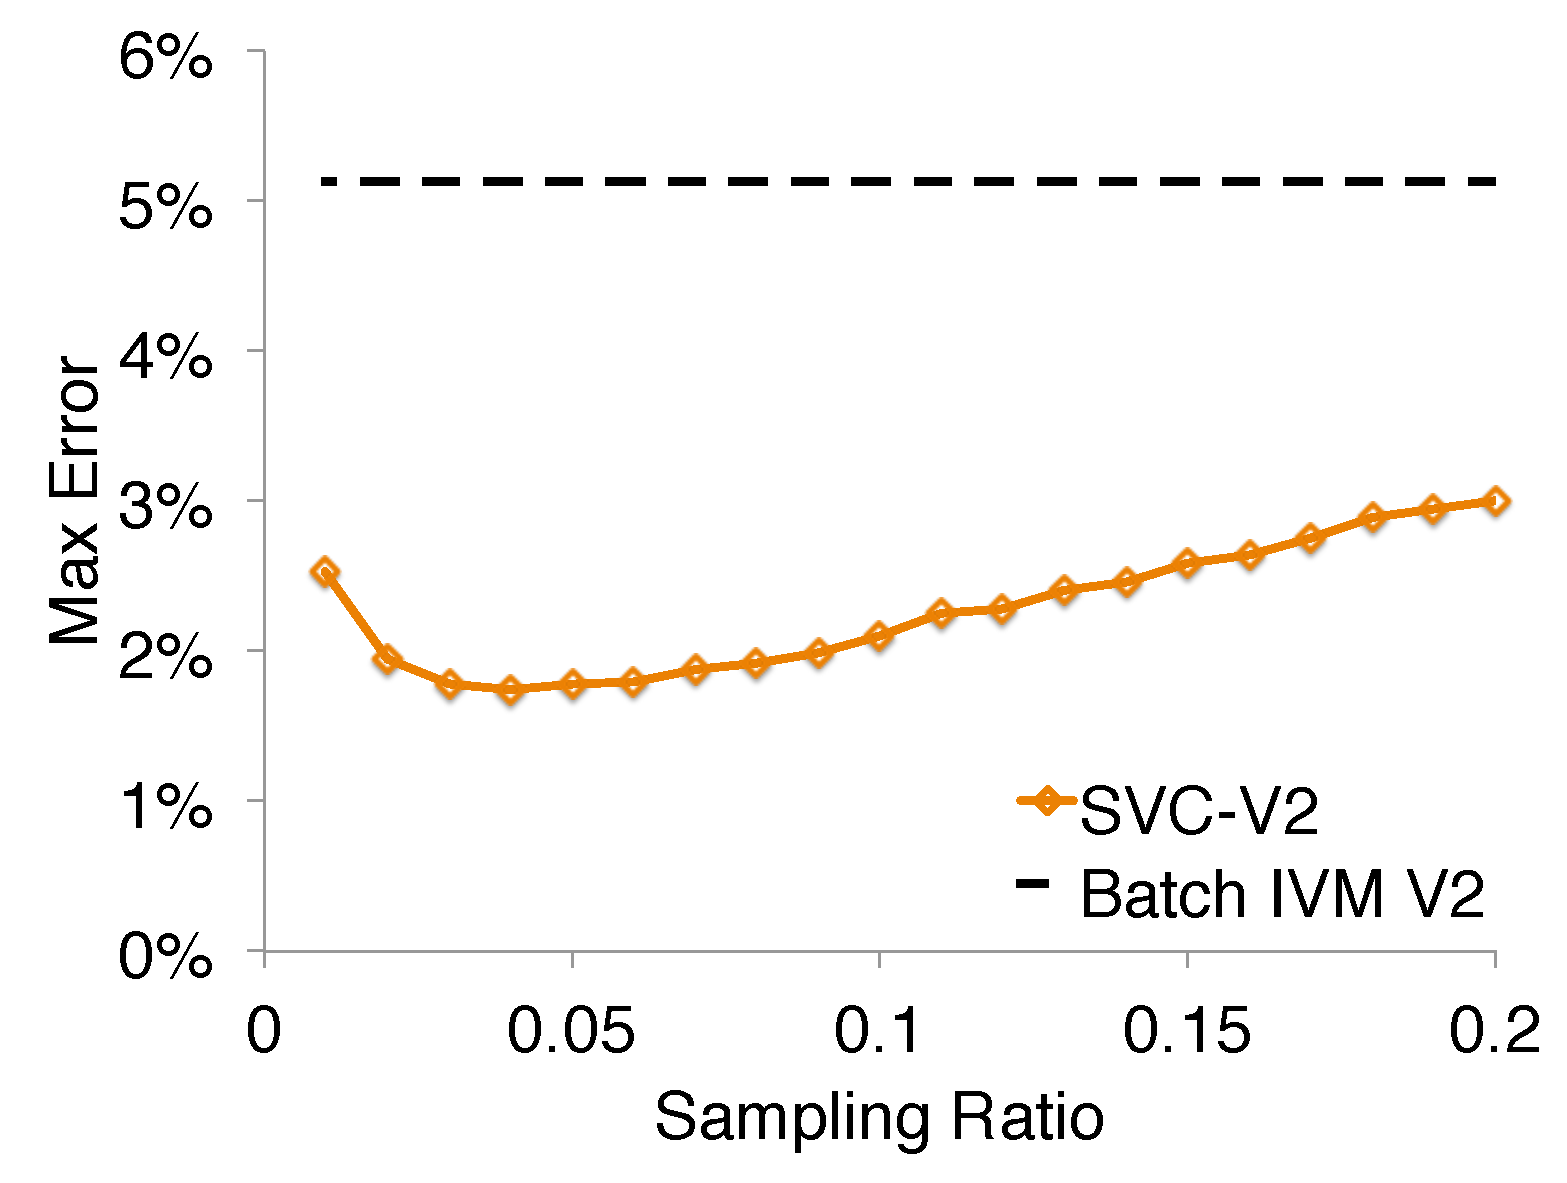
\includegraphics[scale=0.14]{exp/con_5.pdf}
 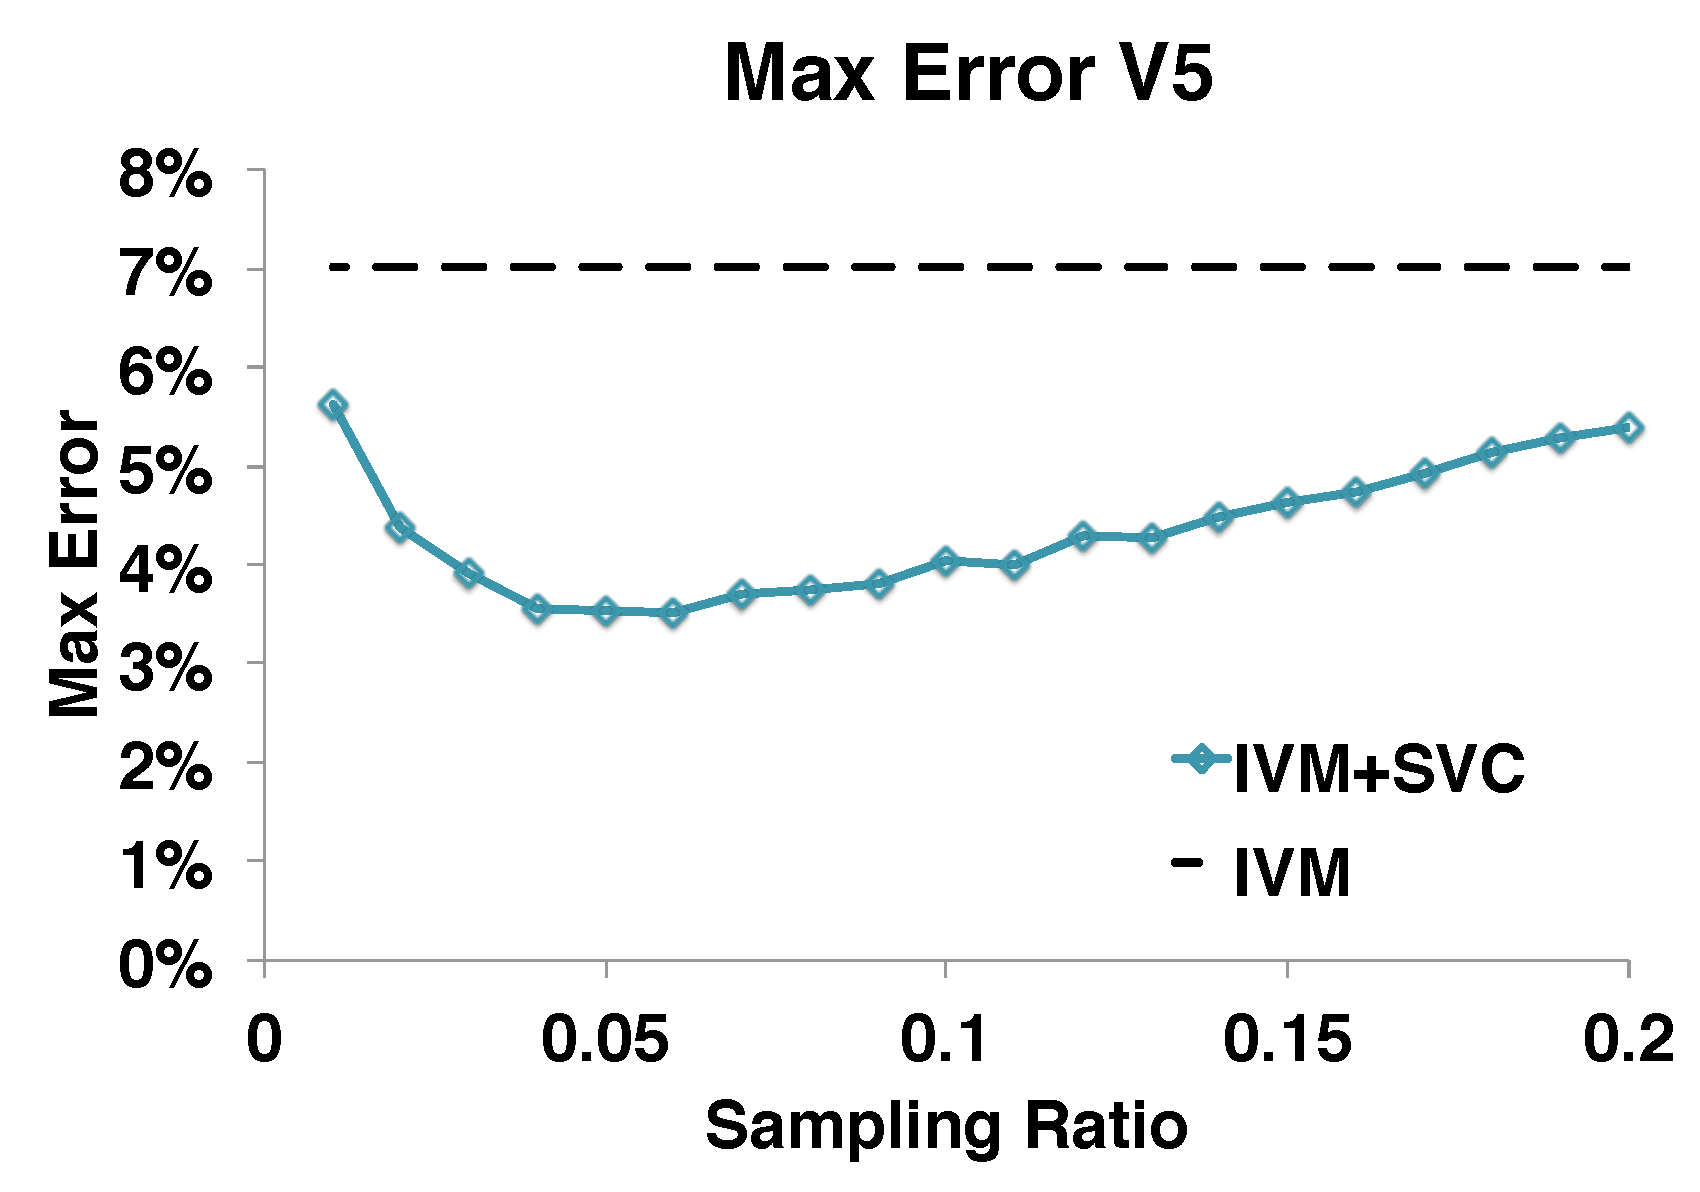
\includegraphics[scale=0.14]{exp/con_6.pdf}
 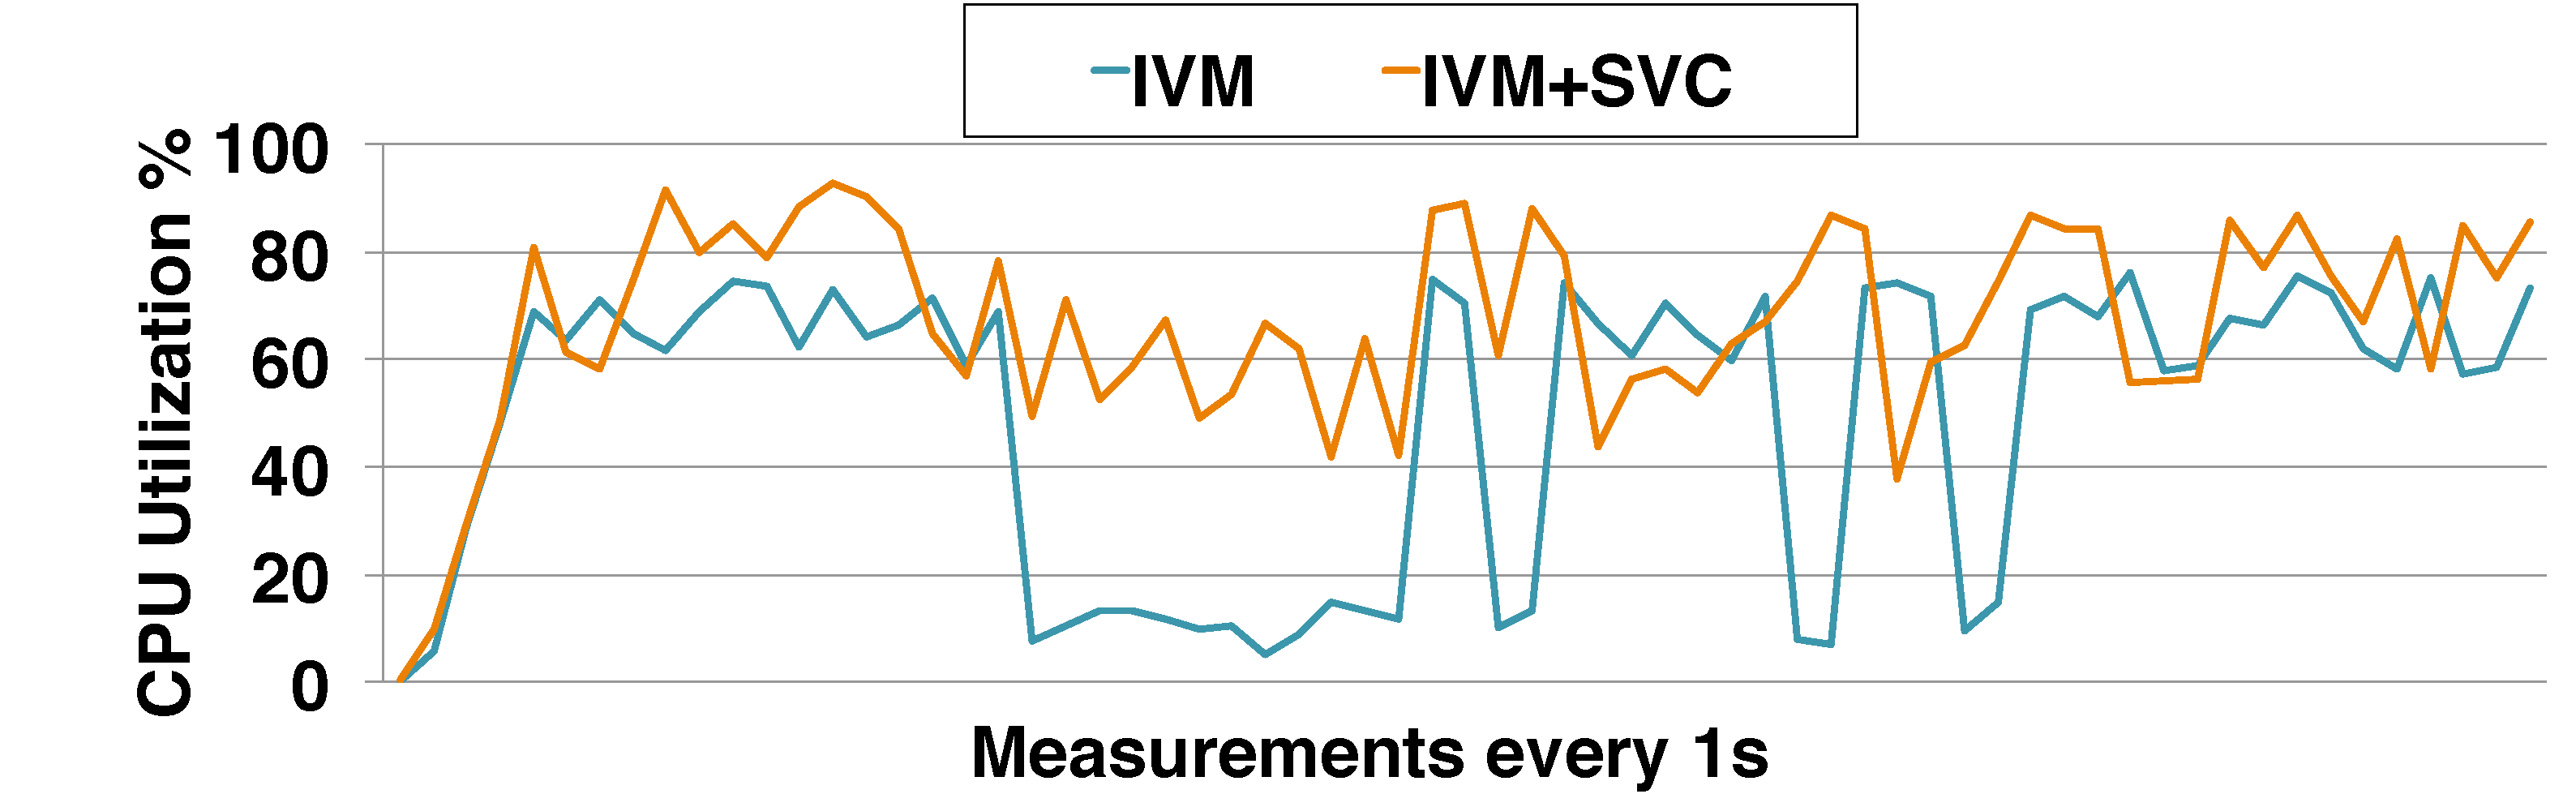
\includegraphics[scale=0.14]{exp/con_7.pdf}
 \caption{TODO}
\end{figure}